\documentclass[11pt,twoside,openright]{book}
\usepackage[paperwidth=170mm,paperheight=240mm,top=20mm,total={130mm,195mm}]{geometry}
% Reccomendations for thesis printing:
% - Write in (a) A4, (b) 170x240 mm.
% - Minimum margin of 2 cm on top and sides, 2.5 on bottom. Page numbers underneath margin. (Is this for a or b?) latex A4 does well above this automatically.
% - Fontsize: (a) 12, (b) 11
% - Numbering: Bottom centered or side aliged (right align odd, left align even numbers)
% - Chapters, table of contents, foreword etc on odd (right) pages.

% Force bibliography to appear in table of contents
\usepackage[nottoc]{tocbibind}

%For the title page pdf
\usepackage{pdfpages}

% For fancy quote
\usepackage{epigraph}

% Fancy chapter headings
\usepackage{titlesec, color}
\definecolor{gray75}{gray}{0.75}
\newcommand{\hsp}{\hspace{20pt}}
\titleformat{\chapter}[hang]{\Huge\bfseries}{\thechapter\hsp\textcolor{gray75}{|}\hsp}{0pt}{\Huge\bfseries}


% For norwegian characters (fontenc also needed for fancy chapter headings).
\usepackage[utf8]{inputenc}
\usepackage[T1]{fontenc}

\usepackage{comment}

% urls
\usepackage[hidelinks]{hyperref}

% Math
\usepackage{amsmath,bm}

% Subfigures etc
\usepackage{graphicx,subcaption}

\usepackage{dirtytalk}

% Reference management
\newcommand{\Eqref}[1]{Eq.~\eqref{#1}}
\newcommand{\Eqsref}[1]{Eqs.~\eqref{#1}}
\newcommand{\Figref}[1]{Fig.~\ref{#1}}
\newcommand{\Figsref}[1]{Figs.~\ref{#1}}
\newcommand{\Secref}[1]{Sec.~\ref{#1}}
\newcommand{\Chapref}[1]{Chapter~\ref{#1}}


\newcommand{\first}{Paper I}

% Bibliography management
\usepackage[numbers,sort,compress]{natbib}
%\bibliographystyle{apsrev4-1}
\bibliographystyle{unsrtnat}


\begin{document}
\frontmatter
\includepdf{figures/PHD_first_page.pdf}

% To ensure: titlepage-blank-epigraph-blank-preface, with preface the first numbered page.
% We start counting from the first page, wiich is the epigraph.
\newpage\null\thispagestyle{empty}\newpage

\setcounter{page}{1}\thispagestyle{empty}\newpage
%\newpage\null\thispagestyle{empty}\newpage

\section*{Abstract}
The exhaust of particles and heat in the boundary of contemporary magnetic confinement experiments remains to this day a major obstacle on the road to
commercially viable fusion energy production. It is recognized, that coherent structures of hot and dense plasma, called blobs or filaments, are the dominant mechanism for cross-field particle transport. These filaments are created by plasma turbulence at the outboard midplane and move radially outwards driven by interchange motions. This leads to high average particle densities and relative fluctuation levels in the scrape-off layer, which increases plasma-wall interactions.

Time series of the plasma density measured at a fixed point using either Langmuir probes or gas puff imaging have shown highly intermittent fluctuations across a variety of devices, plasma parameters and confinement modes. Recent statistical analysis of measurement data time series has revealed that the fluctuations are well described as a superposition of uncorrelated exponential pulses with fixed duration and exponentially distributed pulse amplitudes, arriving according to a Poisson process.  

Due to the complexity of the
physics involved in the boundary of fusion devices, numerical simulations are utilized to gain an accurate description of scrape-off layer plasmas. This approach requires a validation metric for simulations of plasma turbulence such as the statistical framework based on filtered Poisson processes. In this thesis, well-established models for scrape-off layer plasmas are analyzed. These models use two-fluid equations simulating plasma evolution in the two-dimensional plane perpendicular to the magnetic field. Time series of the plasma density are measured at a fixed point and their fluctuation statistics are compared to experimental measurements utilizing the statistical framework. This includes probability density functions, power spectral densities and conditionally averaged waveforms. In addition, simulations of a population of seeded blobs are performed in order to study the effects of blob interactions. It is shown that the fluctuation statistics of single-point measurements in simple numerical models stand in excellent agreement with their experimental counterparts. This work thereby sets a new standard and methodology for validating scrape-off layer turbulence simulations. 





\begin{comment}
Statistical properties of numerical simulations of scrape-off layer (SOL) plasmas are investigated. Single point measurements of the plasma density and temperature of two established fluid models are studied and compared to the predictions of the Filtered Poisson Process (FPP), a phenomenological model describing all major statistical properties of experimental measurements of fluctuations in SOL plasmas.

We find that the idealized interchange model exhibits the statistical properties of SOL
fluctuations and the FPP model only to some extend. The probability density functions (PDF) for the temperature and
radial velocity fluctuations change from a normal distribution in the center
of the simulation domain to a distribution with an exponential tail at higher
radial positions. The power spectral densities (PSD) have an exponential shape which can be attributed to underlying Lorentzian pulses. The time
series of the temperature show periods of strongly intermittent fluctuations
with large bursts, interrupted by quiescent periods of quasi-periodic fluctuations.
This effect can be attributed to the generation of a sheared mean flow through the fluid layer resulting in predator-prey-like dynamics of
the energy integrals.

Analytical work on a shot noise process
with periodic arrivals reveals that the PSD
of this process with Lorentzian pulses and exponentially distributed amplitudes has an exponential shape with a Dirac comb of decaying amplitudes. It is shown that that moderate deviations from perfect periodicity destroys the Dirac comb as it
leads to a broadening of its peaks and the decrease of the peak amplitudes
for higher harmonics, resembling the PSD of the idealized interchange model.

Equivalent analysis on time series of the reduced Braginskii fluid model show that the PDFs of stationary time series of the plasma density have an
exponential tail for high radial positions. The average burst or pulse shape is well described by a
two-sided exponential function. The PSD of the particle density is that of the
average pulse shape and does not change with radial position. The amplitudes
and the waiting times between two consecutive arrivals are exponentially distributed. The results of this model thereby stand in perfect agreement with the predictions of
the FPP model. The
presented statistical framework defines a new validation metric for boundary turbulence simulations.

Lastly, the interaction of filaments in the SOL is investigated in the reduced Braginskii model utilizing a blob tracking algorithm. We observe that a high level of filament interaction  leads to an increase in the average radial velocity, as filaments interact with the electrostatic potential of one another. For all investigated levels of filament interaction, the size-velocity relationship of these structures follow established scaling laws. The relevance of isolated filament simulations for complex turbulence models is thereby displayed.\textcolor{red}{Maybe reduce amount of information since abstract became very long!}
\end{comment}

\newpage\null\newpage
\section*{Acknowledgements}
After three and a half years as a PhD student, I would like to thank a number of people who have supported me on this journey. First, I would like to thank my main supervisor, Odd Erik Garcia.  In addition to his guidance and support, Odd Erik also gave me the opportunity to participate at summer schools at CCFE and MIT, visit DTU for two weeks during my first year and spend a whole year at CCFE. Visiting different research facilities and meeting many gifted scientists was one of the highlights during this time. 

I would also like to thank Fulvio Militello for hosting me at CCFE and proofreading parts of this thesis. Our weekly catch-ups in the last year and a half were extremely insightful and productive. I am grateful to him reserving time for me even though I am not directly supervised by him.

I am very grateful for being part of such friendly and supportive research groups. These include Audun Theodorsen, Ralph Kube, Juan Manuel Losada and Magdalena Korzeniowska at UiT. From CCFE these include John Omotani, Tom Nicholas, Fabio Riva, Sarah Newton and Nick Walkden as well as Matthias Wiesenberger at DTU. Further thanks go to my office mates, Patrick Stoll, Sindre Fritzner, Tuomas Heiskanen, Tom Farley, Daljeet Singh Gahle, Enrique Miralles and Joe Allcock. Raheesty Nishta Nem deserves my gratitude for proof-reading my thesis and giving me valuable comments. I am also grateful to the University of Tromsø – The Arctic University of Norway for funding my PhD. 

On a less academic note, I would like to thank my landlord in Oxford, Michael Butcher, for letting Sajidah and me stay in his flat during the UK-wide lockdown due to the COVID-19 pandemic. Being able to stay together with Sajidah made this challenging time much easier. Thanks also to my friends in Tromsø and Oxford, I have always been looking forward to spending time with you during band practice and other occasions.

Vielen Dank an meine Familie für eure Unterstützung und euer Verständnis für die örtliche Distanz. Auch wenn ich euch pandemiebedingt schon lange nicht mehr persönlich sehen konnte, bleibt ihr in meinem Herzen.

Finally, I would like to thank Sajidah for her patience, laughter and support. This PhD would not have been as joyful without you.
\newpage\null\newpage

\tableofcontents

\mainmatter

% Chapter: First chapter 
\chapter{Fluctuations in magnetized plasmas}
Nuclear fusion is the process by which light atomic nuclei fuse
together to form heavier nuclei and smaller by-products, releasing large amounts of energy. Since the middle of the last century, different strategies to harness fusion energy have been investigated. At present magnetic confinement is considered the most promising approach to deliver fusion power in the foreseeable future. To this day, however, controlling and harnessing nuclear fusion remains one of the greatest engineering challenges. Magnetically confined fusion requires the fuel to have enormously high temperatures while the vessel walls must be at room temperature or lower. The heat exhaust problem has therefore famously been referred to as \say{probably the main challenge towards the realization of magnetic confinement
fusion} \cite{Romanelli2012}. A detailed understanding of the intricate physics involved in the boundary of fusion devices therefore remains crucial in order to provide fusion energy as a sustainable and $\mathrm{CO_2}$ emission free option for the future energy grid.

This thesis project is concerned with numerical simulations of boundary plasmas and a statistical analysis of plasma fluctuations. These simulations require a method of validation with experimental observations. In this thesis, a recently developed stochastic model for fluctuation statistics is utilized to identify suitable numerical models for boundary plasmas.

This thesis is structured as follows: This chapter delivers a brief overview of the current state of knowledge on the boundary of fusion plasmas. The main emphasis will lie on plasma fluctuations for reasons that will become clear over the course of this chapter. Chapter 2 is dedicated to the derivation of reduced fluid models for the boundary plasma, which are used for the numerical simulations presented in this thesis. Chapter 3 introduces the Filtered Poisson Process, a phenomenological model which is able to describe all relevant statistical properties of plasma fluctuations in the boundary region. Chapter 4 delivers a summary of the publications and unpublished manuscripts included in this thesis and Chapter 5 provides the conclusion and outlook. The published papers and unpublished manuscripts are attached at the end of this thesis, representing the main contribution of this work. 

\section{Nuclear fusion}
Although a multitude of nuclear reactions produces fusion energy, only the reaction of the hydrogen isotopes Deuterium ${}_1^2\mathrm{D}$ and Tritium ${}_1^3\mathrm{T}$,
\begin{equation}
	{}_1^2\mathrm{D} + {}_1^3\mathrm{T} \rightarrow {}_2^4\mathrm{He}\,(3.5 \textrm{MeV}) + {}_0^1\textrm{n} \,(14.1 \textrm{MeV}),
\end{equation}
 is feasible with the prevailing technology. This reaction produces a helium particle ${}_2^4\mathrm{He}$ and a neutron ${}_0^1\textrm{n}$ together with $17 \,\textrm{MeV}$ of kinetic energy. This exothermic, single-step reaction has the largest fusion cross section at the lowest temperatures of all potential reactions. In addition, the low atomic number results in a lower electrostatic potential that must be overcome, making this the most promising candidate for fusion power plants. With one in 6420 hydrogen atoms in sea water, Deuterium can be considered abundant, while the radioactive Tritium must be obtained from breeding of the lithium isotope  ${}^6\mathrm{Li}$, which can be found in minerals from the Earth's crust. Due to the high temperature of approximately $10^8\, \mathrm{K}$ for $\mathrm{D}$-$\mathrm{T}$ fusion, no solid vessel could achieve steady-state confinement at these temperatures. The fuel would instantaneously lose its heat when colliding with the vessel walls. In order to achieve long enough energy confinement times, required for producing fusion power in a steady-state, a different approach has to be adopted. Since all hydrogen particles are fully ionized at these temperatures, i.e., in a plasma state, the particles can be confined with magnetic fields \cite{freidberg2008plasma}.

\section{Magnetic confinement}

Magnetic Confinement Fusion (MCF) chooses the approach to use the gyromotion of charged particles in a magnetic field to confine the plasma. An array of cylindrical solenoidal coils creating a uniform magnetic field can confine the plasma in the radial direction, however charged particles moving along these field lines can intersect material surfaces at both ends. The simplest method to mitigate these end losses is to bend the magnetic field to connect the ends, which results in a torus shape. The resulting inhomogeneity of the magnetic field due to its curvature and radial gradient, however, complicates plasma confinement. Since a gyrating particle experiences a stronger magnetic field on one side of its orbit than the other, it will experience a change in its gyration radius, resulting in a net drift which is in opposite direction for ions and electrons. These \say{guiding-center drifts} which are perpendicular to the magnetic field \textbf{B} and its variation $\nabla B$, create a vertical electric field \textbf{E}. The resulting fields give rise to another guiding-center drift, the electric or \textbf{E}$\times$\textbf{B} drift, which moves both negatively and positively charged particles radially outwards. A toroidal plasma current, induced by a central transformer, creates a poloidal magnetic field. Introducing this poloidal field results in helical magnetic field lines, which mitigates this problem since the guiding-center drifts cancel out as the particles rotate poloidally while following the magnetic field lines. Outer poloidal field coils are used in addition to shape and position the plasma column. This concept is known as a tokamak, invented in the 1950s in the Soviet Union and to this day considered to be the most promising route for plasma confinement and nuclear fusion. A schematic illustration of the tokamak concept is shown in \Figref{Fig:tokamak}. 
\begin{figure}[t]
	\centering
	\includegraphics[width=11cm]{figures/tokamak.png}
	\caption{Schematic illustration of a tokamak device \cite{eurofusion}.}
	\label{Fig:tokamak}
\end{figure}

Despite the advanced magnetic geometry of tokamak devices which establish a perfect equilibrium, experimental measurements indicate that large amounts of particles and heat are still transported across the magnetic flux surfaces. This transport is caused by plasma turbulence, which is particularly strong at the boundary of the device. All modern tokamak experiments adopted the \say{divertor configuration}, which is illustrated in \Figref{Fig:sol}. This configuration is achieved by creating a magnetic null point (X-point) in the poloidal plane with a divertor coil carrying a current parallel to the plasma current. Within this point, the magnetic field lines are closed with the last closed flux surface (LCFS), often referred to as the separatrix. The outward region is called the Scrape-Off Layer (SOL), in which the magnetic field lines intersect the divertor plates. Ideally, all plasma leaking from the core through the separatrix into the SOL flows down to the divertor plates where it interacts with the material surfaces, with little to no influence on the fusion process in the core. The poloidal flux expansion near the X-point increases the distance of the magnetic field lines to the divertor plates, letting the plasma cool down before it reaches the material surfaces. Additional precautions, such as tilted target plates, buffers of neutralized gas in front of the target
(divertor detachment) or installing a second divertor above the plasma column (double-null configuration) are applied in some experiments to reduce the heat flux on the divertor plates further. Despite all these efforts, plasma turbulence leads to highly intermittent bursts of particles and heat propagating through the SOL to the main chamber walls, leading to erosion, damages of sensitive equipment and the release of impurities into the core plasma, where they may degrade confinement and create radiative instabilities. An accurate description for the cross-field transport in the SOL is therefore required in order to predict and handle plasma and heat exhaust in future devices \cite{freidberg2008plasma}.
\begin{figure}[t]
	\centering
	\includegraphics[width=11cm]{figures/sol.png}
	\caption{Schematic illustration of the boundary region of a tokamak in a divertor configuration \cite{eurofusion}.}
	\label{Fig:sol}
\end{figure}

\section{Radial transport in the SOL}
 Historically, the first attempts to describe cross-field transport in tokamak plasmas used
 a simple diffusive model in the SOL \cite{connor1999comparison}. In this case the transport follows Fick's law
 \begin{equation}
 	\Gamma_\perp = - D_\perp \frac{\partial n}{\partial r},
 \end{equation}
where $\Gamma_\perp$ stands for the cross-field particle flux, $D_\perp$ is the diffusion coefficient estimated from the plasma parameters \cite{Bohm1949}, $n$ stands for the plasma density and $r$ for the radial/cross field dimension. This model, however, fails to account for experimental observations, requiring significantly higher diffusion coefficients than expected from classical or Bohm diffusion \cite{lipschultz2002investigation,krasheninnikov2008recent}. Experimental radial profiles in the SOL could only be reproduced by numerical simulations by assuming large cross field drifts or high effective diffusion coefficients $D_\perp^\textrm{eff}$, often referred to as \say{anomalous} diffusion \cite{wesson2011tokamaks}. It was expected that the SOL is dominated by strong flows parallel to the magnetic field, transporting most of the plasma to the divertor targets, resulting in exponential profiles with constant $D_\perp^\textrm{eff}$. These assumptions were refuted by experimental measurements such as presented for the TCV tokamak in \Figref{Fig:garcia_fluc}.
  \begin{figure}[t]
	\centering
	\includegraphics[width=8cm]{figures/garcia_fluc.png}
	\caption{Time-averaged, radial profile of the particle density normalized to the separatrix value in the TCV tokamak. The different colored symbols refer to different line-averaged core plasma densities with the black triangles referring to the lowest and the red triangles to the highest value. Reprinted from \cite{garcia2007fluctuations}, with permission from IAEA.}
	\label{Fig:garcia_fluc}
\end{figure}
Here, the variable $\rho$ stands for the distance to the separatrix and the dashed line indicates the beginning of the wall shadow, the region in which the magnetic field lines interact with the vessel walls. For the lowest line-averaged densities $\overline{n}$ a sharp decay in the density profile is observed close to the separatrix, with a much slower decay radially outwards. These regions are referred to as the near-SOL for the region of steep profiles and far-SOL, respectively \cite{labombard2001particle}. For increasing $\overline{n}$ the break point between these two regions moves radially inwards, resulting in a long decay length in the whole SOL, called broadening \cite{militello2016scrape}. This radial variation is also observed in other tokamak experiments such as Alcator C-Mod, MAST, NSTX, ASDEX, JET and DIII-D \cite{umansky1999modeling,rudakov2005far,militello2013experimental,boedo2014edge,carralero2014experimental,stangeby2000plasma,lipschultz2005comparison}, and in numerical simulations with SOL turbulence codes such as ESEL \cite{naulin2007turbulent}. For a purely diffusive transport this effect requires a significant radial increase of the effective diffusion coefficient as indicated in \Figref{Fig:labombard} for Alcator C-Mod plasmas, questioning the concept of purely diffusive transport.
\begin{figure}[t]
	\centering
	\includegraphics[width=8cm]{figures/effective_diff.png}
	\caption{Effective diffusivity profiles for different operational modes of the Alcator C-Mod experiment. The effective diffusion coefficient must vary by several orders of magnitude in order to match purely diffusive transport models. Reprinted from \cite{labombard2000cross}, with the permission of IAEA.}
	\label{Fig:labombard}
\end{figure}
In the case of the DIII-D experiment, UEDGE transport simulations were unable to find any matching diffusion coefficient \cite{pigarov2002tokamak}. This motivates the introduction of an effective anomalous velocity $v_\perp^\textrm{eff}$ to the diffusion model,
\begin{equation}
 	\Gamma_\perp = - D_\perp^\textrm{eff} \frac{\partial n}{\partial r} + v_\perp^\textrm{eff} n.
\end{equation}
For an advective-diffusive transport, however, the particle flux would follow a linear relationship with the inverse density scale length $\lambda_n$ \cite{garcia2007turbulent} as
\begin{equation}
	\frac{\Gamma_\perp}{n} =  v_\perp^\textrm{eff} - \frac{D_\perp^\textrm{eff}}{n} \frac{\partial n}{\partial r} = v_\perp^\textrm{eff} + \frac{D_\perp^\textrm{eff}}{\lambda_n}. 
\end{equation} 
In experimental measurements, such as for TCV shown in \Figref{Fig:garcia_flux}, no linear relationship can be found. Similar studies on the flux–gradient relation in
a simple ESEL interchange model of the SOL at
constant temperatures, shown in \Figref{Fig:naulin},  draw an equivalent conclusion \cite{naulin2007turbulent}.


These findings clearly indicate that a different model is needed in order to describe turbulence and cross-field transport in the SOL adequately. 
\begin{figure}
	\centering
	\begin{minipage}{.48\linewidth}
			\includegraphics[width=\linewidth]{figures/garcia_flux.png}
	\caption{The relationship between the normalized radial particle flux and the inverse density scale length for a range of TCV experiments. Reprinted from \cite{garcia2007turbulent}, with the permission from Elsevier.}
		\label{Fig:garcia_flux}
	\end{minipage}
	\hfill
	\begin{minipage}{.48\linewidth}
		\includegraphics[width=\linewidth]{figures/naulin.png}
	\caption{The flux–gradient relation in a simple ESEL interchange model of the SOL at constant temperatures. Reprinted from \cite{naulin2007turbulent}, with the permission from Elsevier.}
		\label{Fig:naulin}
	\end{minipage}
\end{figure}


\section{Intermittent fluctuations in the SOL}
In the process of finding a better model describing plasma transport in the SOL of tokamak experiments, measurements of the relative fluctuation levels provide additional insight. Among the first experiments investigating this is the Caltech tokamak where fluctuation levels of 10-90\% of the mean were measured in ion saturation current measurements in the edge \cite{zweben1982edge,zweben1983scaling}. Similar observations were made in other experimental devices where these include the TEXT device, shown in \Figref{Fig:wootton}, and in TCV, \Figref{Fig:garcia_rel_fluc}. The fluctuation profiles of the TCV experiment correspond to the time averaged profiles shown in \Figref{Fig:garcia_fluc}. In the low-density case the relative fluctuation levels increase radially in the near SOL and stay approximately constant in the far SOL. Note that the fluctuation levels in the far SOL are independent of the line-averaged core density. For all densities the relative fluctuation levels in the far SOL range between 0.5 and 1, indicating that the broad profiles are dominated by large fluctuations. These findings differ drastically from the plasma core, where fluctuation levels are only around 1\% \cite{mckee2007plasma}. 
\begin{figure}
	\centering
	\begin{minipage}{.48\linewidth}
		\includegraphics[width=\linewidth]{figures/wootton.png}
	\caption{Radial dependencies of fluctuation levels of different plasma parameters in the TEXT tokamak experiment. Reprinted from \cite{wootton1990edge}, with the permission from Elsevier.}
	\label{Fig:wootton}
	\end{minipage}
	\hfill
	\begin{minipage}{.48\linewidth}
		\includegraphics[width=\linewidth]{figures/garcia_rel_fluc.png}
	\caption{Radial profile of the relative fluctuation level of the particle density in the TCV SOL. Reprinted from \cite{garcia2007fluctuations}, with permission from IAEA.}
	\label{Fig:garcia_rel_fluc}
	\end{minipage}
\end{figure}

A more detailed picture of SOL fluctuations can be obtained by analyzing time series of the plasma parameters. These time series are typically obtained by Langmuir probes, consisting of a conducting element which is inserted into the plasma and draws a measurable current \cite{langmuir1923positive,mott1926theory}. Another well-known method is Gas puff imaging (GPI), where a puff of neutral gas is injected into the plasma edge, so that excitation radiation can be measured \cite{zweben2017invited}. Examples for time series measured at the outboard mid-plane in the far SOL of TCV, Alcator C-Mod and KSTAR are shown in \Figref{Fig:time_series}. Here, $\widetilde{\Phi}$ stands for the time series $\Phi(t)$ normalized to have zero mean and unit standard deviation. In all three devices, the time series show strongly intermittent positive bursts, which suggests an explanation for the large relative fluctuation levels in the SOL. A stochastic model describing these fluctuations as a superposition of uncorrelated pulses was introduced in 2012 \cite{garcia2012stochastic}. This phenomenological model, known in the context of stochastic processes as the Filtered Poisson Process (FPP), remains to the day of writing this thesis the most accurate statistical description of SOL fluctuations, as all of its major assumptions and predictions agree with the statistical properties of experimental measurements \cite{garcia2013intermittent,garcia2013burst,garcia2015intermittent,kube2016fluctuation,garcia2017sol,kube2018intermittent,garcia2018intermittent,theodorsen2018universality}. A detailed discussion of the FPP model is provided in Chapter 3 of this thesis.
\begin{figure}[t]
	\centering
	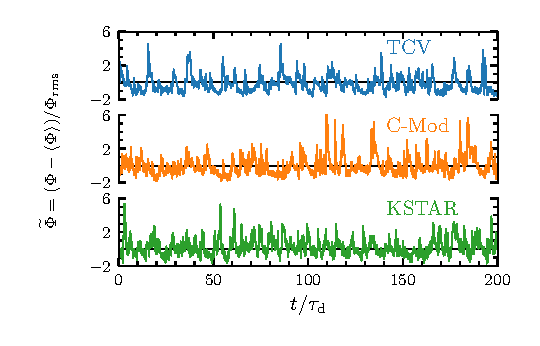
\includegraphics[width=10cm]{figures/compare_ts_alt.eps}
	\caption{Fluctuation time series measured from different tokamak experiments. The time is normalized by the characteristic duration time of the underlying bursts. The black line indicates the mean value of the signal. Image courtesy of A. Theodorsen \cite{theodorsen2018statistical}.}
	\label{Fig:time_series}
\end{figure}

The statistical properties of the fluctuations appear to be remarkably universal across numerous tokamak experiments, confinement modes and plasma parameters. Since positive fluctuations dominate over negative ones, the probability density functions (PDFs) are positively skewed and flattened. \Figref{Fig:antar} shows the PDFs of the ion saturation current measured in the boundary of four different devices, exhibiting almost identical results.  Time series obtained at different radial positions in the boundary region of Alcator C-Mod exhibit close to normal distributions near the separatrix, whereas in the far SOL show increasingly skewed PDFs with an exponential tail towards positive values, as shown in \Figref{Fig:theodorsen_pdf}. Collectively, all of these PDFs are well described by a Gamma distribution with a shape parameter depending on the intermittency of the time series \cite{theodorsen2017relationship}. PDFs with exponential tails towards positive events have also been observed in multiple other devices such as TCV, Tore Supra and KSTAR \cite{antar2001turbulence,antar2003universality,graves2005self,garcia2007fluctuations,garcia2007collisionality,garcia2009blob,garcia2017sol}. The skewness and kurtosis of these time series are exceeding 0 and 3 respectively, as they would be for a normal distribution. A parabolic relationship between skewness and kurtosis has been demonstrated in  \cite{labit2007universal,sattin2009statistics,sattin2009parabolic} which remains consistent with predictions of the FPP model \cite{garcia2016stochastic}.
\begin{figure}
	\centering
	\begin{minipage}{.48\linewidth}
		\includegraphics[width=\linewidth]{figures/antar.png}
		\caption{PDF of the ion saturation current in the boundary of Tora Supra, Alcator C-Mod, MAST and PISCES. Reprinted from \cite{antar2003universality}, with permission from AIP Publishing.}
		\label{Fig:antar}
	\end{minipage}
	\hfill
	\begin{minipage}{.48\linewidth}
		\includegraphics[width=\linewidth]{figures/theodorsen_pdf.png}
		\caption{PDFs of gas puff imaging data time series at different radial positions in the boundary of Alcator C-Mod. The full lines represent the predictions of the FPP model. Reprinted from \cite{theodorsen2017relationship}, with permission from IAEA.}
		\label{Fig:theodorsen_pdf}
	\end{minipage}
\end{figure}

The universality of plasma fluctuations in the SOL is also observed in the power spectral densities (PSDs) of the measured time series \cite{pedrosa1999empirical,carreras1999characterization,theodorsen2017relationship,theodorsen2018universality,kube2018intermittent,garcia2018intermittent}. The PSDs of time series for the ion saturation current in a variety of devices are shown in \Figref{Fig:pedrosa}. For a given scaling factor for the frequency axis all PSDs collapse to a single curve. In contrast to the PDFs, the radial position does not seem to have any influence on the PSDs as shown for Alcator C-Mod in \Figref{Fig:theodorsen_psd}. In all experimental measurements the PSD remains flat for low frequencies and shows a power law decay for high frequencies. The analysis of these fluctuations utilizing the FPP framework has shown that the shape of the PSD can be attributed to the shape of the underlying pulses from the time series \cite{garcia2017auto}, providing further support for the stochastic model.
\begin{figure}
	\centering
	\begin{minipage}{.48\linewidth}
	\includegraphics[width=\linewidth]{figures/pedrosa_psd.png}
	\caption{PSDs of fluctuation time series of the ion saturation current in various devices. Reprinted figure with permission from \cite{pedrosa1999empirical}. Copyright (1999) by the American Physical Society.}
	\label{Fig:pedrosa}
	\end{minipage}
	\hfill
	\begin{minipage}{.48\linewidth}
		\includegraphics[width=\linewidth]{figures/theodorsen_psd.png}
		\caption{PSDs for gas puff imaging time series at different radial positions in the edge of Alcator C-Mod. The broken line shows the FPP predictions. Reprinted from \cite{theodorsen2017relationship}, with permission from IAEA.}
		\label{Fig:theodorsen_psd}
	\end{minipage}
\end{figure}

Apart from stochastic modeling, conditional averaging can be applied in order to reveal the shape of these large-amplitude fluctuations. Hereby all events above a certain threshold, typically 2.5 times the rms-value above the signal mean, are considered and their peak is stored within a time window. The average over all windows is referred to as the conditionally averaged waveform, showing a sharp peak with a short rise and longer decay \cite{antar2003universality,boedo2005edge,garcia2007fluctuations,garcia2007collisionality,garcia2013intermittent,garcia2015intermittent,garcia2017sol,kube2018intermittent,garcia2018intermittent}. The conditionally averaged waveform of time series acquired from the boundary of TCV are shown in \Figref{Fig:garcia2007}. The shape of these large-amplitude fluctuations remain similar for all line-averaged core densities of the experiment and are reproducible by numerical simulations of the two-dimensional ESEL model. \Figref{Fig:theodorsen_CA} shows the agreement of conditionally averaged waveforms for time series measured in different tokamak experiments and compared to an asymmetric, two-sided exponential function. Both the distribution of the maximal amplitude of the conditional structures and the waiting times between two consecutive peaks are found to be exponentially distributed \cite{antar2005scaling,garcia2015intermittent,kube2018intermittent,garcia2017sol,garcia2018intermittent}.
\begin{figure}
	\centering
	\begin{minipage}{.48\linewidth}
		\includegraphics[width=\linewidth]{figures/garcia2007.png}
		\caption{Conditionally averaged waveform of particle density time series from TCV and ESEL simulations. Reprinted from \cite{garcia2007fluctuations}, with permission from IAEA.}
		\label{Fig:garcia2007}
	\end{minipage}
	\hfill
	\begin{minipage}{.48\linewidth}
		\includegraphics[width=\linewidth]{figures/compare_cav_wf.eps}
		\caption{Conditionally averaged waveform for time series measured in the edge of TCV, Alcator C-Mod and KSTAR. The broken line shows a two-sided exponential fit. Image courtesy of A. Theodorsen \cite{theodorsen2018statistical}.}
		\label{Fig:theodorsen_CA}
	\end{minipage}
\end{figure}

In conclusion, the statistical properties of time series measured at the mid-plane boundary of tokamak devices indicate that the SOL is dominated by intermittent structures. In order to investigate the shape of these objects and to gain more information about the physical mechanisms responsible for their transport, stochastic modeling alone, however, does not suffice. 

\section{Plasma filaments}
2D imaging diagnostics such as GPI and wide angle visible imaging reveal that edge transport in the SOL can be attributed to coherent structures. These objects have historically been featured under a variety of names, such as intermittent plasma objects (IPOs), avaloids, solitary vortices and streamers, but are most commonly referred to as filaments or blobs in recent literature. First observations of plasma filaments were made with fast cameras at the Caltech tokamak in the mid 1980's \cite{zweben1985search,zweben1985structure,park1987sj} and with 2D probe arrays in the 1990's \cite{endler1995measurements,endler1999turbulent}. The importance of filaments for edge transport, however, has only been considered at the discovery of the main chamber recycling regime at Alcator C-Mod in 1998 \cite{umansky1998comments}. Since then, plasma filaments have been observed in over 40 devices, including all major tokamak experiments, with a variety of diagnostics \cite{d2011convective}. Filaments typically have a significantly higher density than the surrounding plasma and are aligned to the local magnetic field with their scale lengths much larger in the direction parallel to the magnetic field compared to the perpendicular direction. Filaments have a cross-field size 
between 2 mm and 10 cm, radial velocity of 0.2 to 2 km/s and a lifetime in the range of tens of $\mu$s \cite{kirk2016mode,dudson2008experiments,zweben2002edge,kube2013blob,myra2006blob,boedo2001transport,silva2004fluctuation,carralero2015experimental,muller2009studies}. Examples of plasma filaments for different confinement modes in the MAST device are shown in \Figref{Fig:ayed}. The elongation of the filaments along the magnetic field, stretching from the upper to the lower divertor is clearly visible.  
\begin{figure}[t]
	\centering
	\includegraphics[width=13cm]{figures/ayed_mast.png}
	\caption{Wide angle fast visible imaging of inter-ELM, L-mode and ELM
		filaments in the MAST device. The panels above show the toroidal variation in emission across
		the center column, the peaks are used to label the filaments. Reprinted from \cite{ayed2009inter}, © IOP Publishing.  Reproduced with permission.  All rights reserved.}
	\label{Fig:ayed}
\end{figure}
Filaments propagate through the SOL due to interchange motion, illustrated in \Figref{Fig:xu}. A simplified model ignoring parallel dynamics explains filament motion as follows: Due to the magnetic geometry at the outboard mid-plane, magnetic gradient and curvature drifts result in a charge polarization, perpendicular to the magnetic field \textbf{B}. This results in an electric field \textbf{E}, transporting the filament in the radial direction with the \textbf{E}$\times$\textbf{B} velocity \textbf{u}$_E$. While the filaments propagate outwards they carry particles and heat much faster than purely diffusive transport would allow, explaining the broad profiles in the SOL.
\begin{figure}[t]
	\centering
	\includegraphics[width=10cm]{figures/xu.png}
	\caption{Illustration of charge separation in the filament and the resulting \textbf{E}$\times$\textbf{B} drift, transporting the filament in the radial direction. Reprinted from \cite{xu2010intermittent}, with the permission from AIP Publishing.}
	\label{Fig:xu}
\end{figure}
\Figref{Fig:maqueda} shows an example of a filament propagating through the SOL of NSTX. Here, the filament is visualized in the plane perpendicular to the field lines. Due to their appearance in the two-dimensional plane, filaments are often referred to as blobs in this context.
\begin{figure}[t]
	\centering
	\includegraphics[width=13cm]{figures/maqueda.png}
	\caption{Propagation of a blob from the main plasma through the SOL in the NSTX device. Each box shows a $24\times24$ cm portion of the edge at the outer mid-plane and the frame rate is $7 \mu $s. The position of the separatrix is given by the full line and the the wall shadow by the broken line. Reprinted from \cite{maqueda2011intermittency}, with the permission from Elsevier.}
	\label{Fig:maqueda}
\end{figure}

Measurements using Langmuir probes and GPI simultaneously confirmed that propagating filaments are the same structures that cause intermittent bursts in the time series \cite{grulke2014experimental,zweben2015edge}.  The intermittency of the time series and the length and amplitude of individual bursts are therefore given by the filament parameters. 

Even though radial blob propagation can be qualitatively understood with the presented two-dimensional model, parallel dynamics must be considered for a more accurate picture \cite{krasheninnikov2008recent}. Since the filament plasma is neutral, the current due to magnetic gradient and curvature drifts must be closed. The charged particles stream along the magnetic field lines until they reach the target plates where the resulting parallel current can close in the plasma Debye sheath. The parallel resistivity of the plasma and the sheath resistivity  limits the magnitude of the parallel current. Alternatively, the current can be closed by polarization currents in the cross-field plane, thereby creating the dipolar electric potential. A schematic illustration of the current paths are shown in \Figref{Fig:krasheninnikov}. The ratio of the current closed through the parallel and perpendicular path determines the strength of the electric field in the filament and therefore its \textbf{E}$\times$\textbf{B} velocity. If the parallel currents are dominant and close mainly in the plasma sheath the filament is said to be in the \say{sheath limited} regime, while in the case where the currents are closed in the cross-field plane, the filament is in the \say{inertial} regime. Analytical velocity scaling laws show that the radial velocity of a filament $v_\perp$ is strongly dependent on its perpendicular size $a$ of a filament \cite{theiler2009cross, angus2012effects}, as
\begin{equation}
	v_\perp(a)  \propto	\begin{cases} 
		\sqrt{2 a} \,\, \textrm{for}\,\, a \gg a^*\\
		1/a^2 \,\, \textrm{for}\,\, a \ll a^*
	\end{cases}	
\end{equation}
where $a^*$ is defined as 
\begin{equation}
	a^* = \left(\frac{4 L^2}{\rho_s R}\right)^{1/5}\rho_s.
\end{equation}
In this expression $L$ stands for the connection length to the divertor targets, $R$ is the major radius of the tokamak and $\rho_s$ the ratio between the acoustic speed and the ion gyration radius. These velocity scaling laws are reproduced with numerical simulations \cite{garcia2006radial,kube2012effect,kube2016amplitude}. However, it is found difficult to match these laws to experimental observations in both asymptotic limits, as small filaments are difficult to identify and filaments cannot become larger than the SOL width \cite{myra2006blob,kube2013blob}. Relatively good agreement has been found in the toroidal plasma device TORPEX shown in \Figref{Fig:theiler}, showing the joint probability of the filament velocity and cross-field size \cite{theiler2009cross}. Here, the perpendicular width of the filaments is normalized by $a^*$ and the filament velocity by
\begin{equation}
	v^* = \left(\frac{2 L \rho_s^2}{R^3}\right)^{1/5} c_s
\end{equation} 
with $c_s$ standing for the ion sound speed.
The dashed and dotted lines show the ideal scaling laws for the inertial and sheath connected regimes. It is found that the cross-field size of filaments is in between the scale length of the plasma pressure gradient and the particle gyration radius, hence, filaments are often referred to as mesoscale structures.
\begin{figure}
	\centering
	\begin{minipage}{.48\linewidth}
		\includegraphics[width=\linewidth]{figures/krasheninnikov.png}
		\caption{Schematic illustration of current paths within a filament. Reprinted from \cite{krasheninnikov2008recent}. Copyright © Cambridge University Press 2008.}
		\label{Fig:krasheninnikov}
	\end{minipage}
	\hfill
	\begin{minipage}{.48\linewidth}
		\includegraphics[width=\linewidth]{figures/theiler.png}
		\caption{Joint probability of the normalized filament velocity and cross field size in the TORPEX device. Reprinted figure with permission from \cite{theiler2009cross}. Copyright (2009) by the American Physical Society.}
		\label{Fig:theiler}
	\end{minipage}
\end{figure}

Even though filament generation has been extensively studied in tokamak plasmas \cite{terry2005transport,agostini2007study}, simple toroidal plasmas \cite{theiler2008role,muller2007plasma,furno2008experimental,furno2008mechanism} and numerical simulations \cite{garcia2004computations,bisai2005edge,russell2007collisionality,russell2009saturation}, to this day no quantitatively accurate analytical model of filament generation has been developed \cite{d2011convective, krasheninnikov2007generation, krasheninnikov2008dynamics}.  A number of linear instabilities have been identified that are attributed to cause filament generation, namely the interchange, drift-wave, Kelvin-Helmholtz, Rayleigh–Taylor, resistive-ballooning and conducting-wall instabilities \cite{d2011convective,manz2015origin}. Due to the limited understanding of the intricate physics responsible for filament generation in tokamak plasmas, this topic remains a field of active research. 

\section{Numerical modeling of SOL plasmas}
As experimental measurements and analytical models for SOL turbulence and plasma filaments face intrinsic limitations, numerical simulations of first principle based models have provided further insight. Due to the complexity of the involved physics, it remains a delicate task to derive models with appropriate approximations that still capture the most relevant physical mechanisms of SOL turbulence. Attempts to model the SOL with gyrokinetic particle-in-cell codes are limited by their enormous computational costs and their dependence on poorly understood boundary conditions \cite{chang2008spontaneous,churchill2017pedestal}. Electromagnetic gyrofluid models have been derived \cite{madsen2013full} and applied for studying temperature dynamics and finite Larmor radius effects on filaments \cite{wiesenberger2014radial,held2016influence}, as well as turbulence in open and closed magnetic field lines \cite{ribeiro2005tokamak,ribeiro2008gyrofluid}. At present, most numerical models for SOL turbulence and filament dynamics originate from the standard plasma fluid transport equations derived by Braginskii \cite{braginskii}. The derivations of the fluid models used in the papers and manuscripts included in this thesis are discussed in Chapter 2. 

Numerical simulations of SOL plasmas can be categorized into models of saturated turbulence where filament-like structures are created due to nonlinear dynamics, and simulations of explicitly seeded,  isolated filaments. The first self-consistent evolution of a seeded plasma blob in two dimensions has been studied in 2003 \cite{bian2003blobs}, shown in \Figref{Fig:bian}. Here, the blob is initialized as a symmetrical 2D-Gaussian on a constant plasma background. The radial propagation and the evolution of the blob into a mushroom-shaped object with a steep front has been observed.  The radial variation of the density of the blob and its according \textbf{E}$\times$\textbf{B} velocity is shown in \Figref{Fig:garcia_1}. The peak of the radial velocity is trailing the density peak, resulting in a steepening of the blob front. The according temporal evolution is shown in \Figref{Fig:garcia_2}, where the observed pulses have a short rise and long fall time; an observation consistent with the underlying pulses of time series in experiments such as in \Figref{Fig:time_series}. Studies of isolated filaments have been extended to three dimensions, considering dynamics parallel to the magnetic field \cite{angus2012effect,walkden2013characterization,easy2014three,easy2016investigation,militello2016multi,riva2016blob} and have been used to investigate specific physical effects such as electromagnetic effects or finite ion Larmor radius effects \cite{angus2012effect,lee2015electromagnetic,gingell2012transport,gingell2014plasma}. Models for radial blob velocity dependencies on filament amplitudes and sizes have been developed \cite{garcia2005mechanism, garcia2006radial,kube2011velocity,kube2016amplitude}. Simulations of multiple simultaneously seeded filaments discovered that filaments in close proximity interact through the electric potential they generate \cite{militello2017interaction,kendl2018gyrofluid}. A systematical analysis of blob interaction in dependence of the intermittency, defined as the level of blob overlap, is presented in Paper IV.
\begin{figure}[t]
	\centering
	\includegraphics[width=6cm]{figures/bian.png}
	\caption{Contour  plot  of  the  evolution  of  a  2D  density  blob. Reprinted from \cite{bian2003blobs}, with the permission from AIP Publishing.}
	\label{Fig:bian}
\end{figure}
\begin{figure}
	\centering
	\begin{minipage}{.48\linewidth}
		\includegraphics[width=\linewidth]{figures/garcia_blob_1.png}
		\caption{Radial variation of the plasma density (full line) and the radial velocity (broken line) at the symmetry axis of a seeded blob. Reprinted from \cite{garcia2005mechanism}, with the permission from AIP Publishing.}
		\label{Fig:garcia_1}
	\end{minipage}
	\hfill
	\begin{minipage}{.48\linewidth}
		\includegraphics[width=\linewidth]{figures/garcia_blob_2.png}
		\caption{Temporal evolution of the plasma density recorded at the symmetry axis at different radial positions. Reprinted from \cite {garcia2005mechanism}, with the permission from AIP Publishing.}
		\label{Fig:garcia_2}
	\end{minipage}
\end{figure}

First attempts of modeling plasma turbulence typically use two-dimensional slab geometries, where curvature effects are modeled by effective gravity terms. Rayleigh–Bénard convection models have been used as a simplified description of the non-linear interchange dynamics in the
SOL \cite{pogutse1994resistive,beyer1996center,horton1996turbulent,berning2000bifurcations,garcia2003confinement,garcia2003bursting,garcia2006two,decristoforo2020intermittent}. These models have been further extended by including sheath dissipation due to losses along magnetic field lines and drift wave dynamics in the edge region \cite{benkadda1994interchange,sarazin1998intermittent,naulin1999dispersion,garcia2001two,ghendrih2003theoretical,sarazin2003theoretical,garcia2004computations,bisai2004simulation,garcia2005turbulence,bisai2005formation,garcia2006turbulence}. One example for a turbulence simulation in a 2D slab geometry of a model including sheath dissipation is presented in \Figref{Fig:decristoforo}. Plasma streaming from the core into the SOL is modeled as a density source term in the left hand side of the simulation domain. Small perturbations in the plasma density become unstable and result in coherent structures that propagate radially outwards due to the interchange mechanism. The transition from closed to open magnetic field lines is simulated by applying different closures for the parallel dynamics. These 2D turbulence simulations have contributed to the understanding of the stability of filaments in the SOL and were able to reproduce the characteristic PDFs of plasma fluctuations and their radial variations \cite{garcia2005turbulence,militello2012simulations}. Further investigations on the statistical properties in turbulence simulations can be performed by analyzing time series \cite{,naulin2003electromagnetic,naulin2004statistical,garcia2007fluctuations,decristoforo2020intermittent,decristoforo2021numerical} and blob tracking methods in order to investigate filament properties \cite{nespoli2017blob,nespoli20193d,paruta2019blob,decristoforo2020blob}.
\begin{figure}[t]
	\centering
	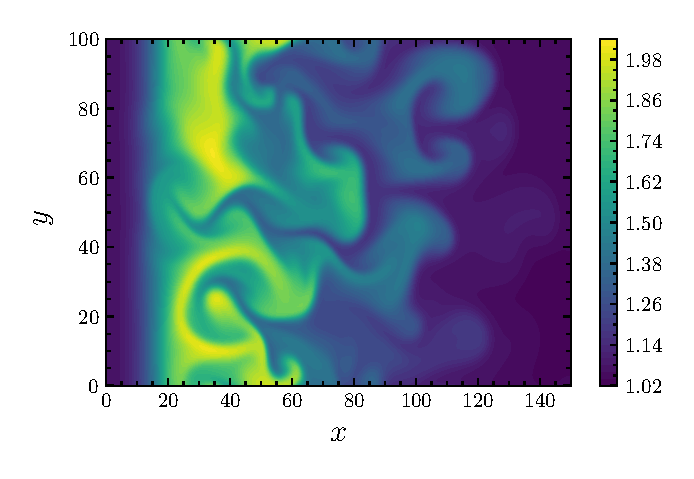
\includegraphics[width=10cm]{figures/decristoforo.eps}
	\caption{Snapshot of plasma density of a two-dimensional turbulence simulation. Plasma is injected into the simulations domain at a constant rate and generates blob-like structures due to turbulence. Reprinted from \cite{decristoforo2020blob}, with the permission from AIP Publishing.}
	\label{Fig:decristoforo}
\end{figure}

Advances in computing power enabled three-dimensional turbulence simulations in the last decade, taking into account the parallel dynamics in SOL plasmas \cite{naulin2005shear,ricci2012simulation,tamain20143d,easy2016investigation,dudson2017hermes,stegmeir2018grillix,Nicholas2021comparing}. Three-dimensional simulations enable implementing realistic geometries and can therefore be used to explore X-point effects and different divertor configurations \cite{nespoli20193d,riva2019three}. Due to their immense computational costs, three-dimensional turbulence simulations have relatively short runs, limiting the amount of statistical analysis that can be performed. 

A variety of comparisons between the output from numerical simulation codes and experiments have been performed in order to validate simulation codes. These studies mainly focused on the dynamics of individual blob
structures or on specific physical effects on turbulence and transport. Surprisingly little attention has been attributed to comparisons of fluctuation statistics, considering their universal nature in experiments. The published papers and yet unpublished manuscripts included in this thesis attempt to fill this gap. Here, the main focus lies on utilizing the FPP model, which predicts all major statistical properties of experimental measurements at the outboard mid-plane. By comparing time series from numerical simulations to the predictions of the FPP model one can identify which parameters and assumptions conform to experimental observations. We can thereby gain additional insight and a better understanding of the intricate physics of the boundary of present and future fusion devices.




% Chapter: Second chapter 
\chapter{Reduced fluid models for SOL plasmas}
In this chapter, a brief derivation of the reduced fluid models used in the included publications is presented. The derivations start from the Braginskii fluid equations whose assumptions and validity for SOL plasmas are discussed. Applying drift reduction, Bohm-normalization and a number of approximations, results in the reduced two-fluid model, equivalent to the two-dimensional fluid models used in Paper III and IV. By applying interchange normalization this model will be further modified to the idealized interchange model, used in Paper I. 

\section{Braginskii fluid equations}
The Braginskii fluid model is derived by taking successive velocity moments of the kinetic Boltzmann equation and applying a collisional closure. Each moment depends on the next higher order and therefore require additional assumptions to obtain a closure for the model. The Braginskii equations describe the evolution of the three lowest order fluid moments. The assumptions and the formulation of this closure are presented in \cite{braginskii}. The standard Braginskii fluid equations describing the evolution of the particle density $n_\alpha$, fluid velocity $\textbf{u}_\alpha$ and temperature $T_\alpha$ for particle species $\alpha$ are given by 
\begin{equation}\label{brag_1}
	\frac{\partial n_\alpha}{\partial t} + \nabla \cdot (n_\alpha \textbf{u}_\alpha) = 0,
\end{equation}
\begin{equation}\label{brag_2}
	m_\alpha n_\alpha \left(\frac{\partial}{\partial t} + \textbf{u}_\alpha \cdot \nabla\right)\textbf{u}_\alpha = - \nabla p_\alpha - \nabla \cdot \Pi_\alpha +Z_\alpha e n_\alpha\left(\textbf{E} + \textbf{u}_\alpha \times \textbf{B}\right) + \textbf{R}_\alpha ,
\end{equation}
\begin{equation}\label{brag_3}
	\frac{3}{2}n_\alpha \left(\frac{\partial}{\partial t} + \textbf{u}_\alpha \cdot \nabla\right)T_\alpha + p_\alpha \nabla \textbf{u}_\alpha = - \nabla \cdot \textbf{q}_\alpha - \Pi_\alpha : \nabla \textbf{u}_\alpha + Q_\alpha.
\end{equation}

Here, $\alpha$ determines the particle species, i.e., electrons and ions, $m$ the particle mass, $p$ the pressure, $Z_\alpha e$ the particle charge, $\textbf{R}$ the friction force, $\Pi$ the viscous stress tensor, $\textbf{q}$ the heat flux, : the tensor inner product and $Q$ the frictional interspecies heating and energy exchange.%, and $S$, $\textbf{S}$ and $W$ represent local density, momentum and energy sources, respectively.
%In the following, we will focus on the first two moments as all models used in the included papers are isothermal. 

The Braginskii equations are only applicable if certain assumptions for the modeled system are valid. Applying fluid equations requires that the distribution of particle velocities is close to Maxwellian, i.e., the time scale of relaxation back to a Maxwellian must be shorter than the characteristic time scales of the modeled system. If this condition is fulfilled, the system is referred to as collisional. %This can be expressed as $\omega_c \ll \nu_{ei}$ and $\omega_c \ll \nu_{ii}$ where $\omega_c$ stands for the characteristic frequency of the modeled system and $\nu_{\alpha\beta}$ for the average collision frequency between particle species $\alpha$ and $\beta$. In addition, $l_\parallel \gg \lambda_e$ and $l_\perp \gg \lambda_i$ where $l_\parallel$ and $l_\perp$ represent the smallest length scales of the system parallel and perpendicular to the magnetic field and $\lambda_\alpha$ is the mean free path for a particle species $\alpha$, given by $\lambda_\alpha = v_{\mathrm{th},\alpha}/\nu_{\alpha\beta}$ with the thermal velocity defined as $v_{\mathrm{th},\alpha}= \sqrt{T_\alpha/m_\alpha}$. \textcolor{red}{Ask Fulvio about  i and e}
In addition to being collisional, a plasma must be strongly magnetized to be adequately described by the Braginskii equations. This implies that the particles complete many gyrations between collisions, setting an upper limit for the collisionality of the plasma. %This condition can be formulated as $\nu_{ie} \ll \Omega_e$ and $\nu_{ii} \ll \Omega_i$ where the gyration frequency is defined as $\Omega_\alpha = eB/m_\alpha$, and $l_\parallel \gg \rho_e$ and $l_\parallel \gg \rho_i$ with the gyration radius given by $\rho_\alpha = v_{\mathrm{th},\alpha}/\Omega_\alpha$. These conditions define the range of time and length scales in which the Braginskii model is valid.

In summary, the phenomenon we want to model needs to satisfy the following conditions in order to be well described by the Braginskii equations:
\begin{equation}
	L_\perp \gg \rho_\alpha,
\end{equation}
\begin{equation}
	L_\parallel \gg \lambda,
\end{equation}
\begin{equation}
	\tau \gg \tau_c \gg \Omega_\alpha^{-1}. 
\end{equation}
In these expressions $L_\perp$ stands for the characteristic size of the modeled phenomena perpendicular to the magnetic field, $\rho_\alpha$ is the gyration radius for species $\alpha$, $L_\parallel$ the parallel size of the system, $\lambda$ the collisional mean free path, $\tau$ the characteristic time of the problem, $\tau_c$ the collision time and $\Omega_\alpha$ the gyration frequency of the referred particle species \cite{militellobook}. 

For the further derivation using drift reduction it will be useful to quantify the magnetization. We thereby define the magnetization parameter $\delta$ as 
\begin{equation}
	\delta = \frac{\rho_\alpha}{L_\perp}.
\end{equation}
The magnetization can be equivalently expressed in the temporal domain by 
\begin{equation}
	\delta = \frac{\nu_{ie}}{\Omega_i}
\end{equation}
where $\nu_{ie}$ stands for the collisional frequency between ions and electrons.

For both electrons and ions the magnetization parameter is $\delta \ll 1$ for a fully magnetized plasma. 


\section{Drift reduction}
The Braginskii model given by \Eqsref{brag_1} - \eqref{brag_3} is very general, making modeling of SOL plasmas with the presented equations relatively inefficient. A more suitable description of plasma phenomena in the SOL can be derived by simplifying the presented model with an approach called drift ordering. Since turbulence and filaments in the SOL, evolve with velocities much lower than the plasma sound speed $c_s = \sqrt{(T_e+T_i)/m_i}$ we apply the ordering
\begin{equation}
	\textbf{u}_\perp \sim \frac{\rho_\alpha}{L_\perp} c_s \sim \delta c_s.
\end{equation}
This ordering assumes that the transverse electric fields are small, resulting in the perpendicular electric field being substantially electrostatic. This is a direct consequence of the $\textbf{E}\times\textbf{B}$ velocity being a factor $\delta$ smaller than sound speed and Faraday's law \cite{militellobook}. We can now determine the perpendicular part of the momentum equation, given by \Eqref{brag_2}, by taking the cross product with $\textbf{B}$ resulting in
\begin{equation}
	\textbf{u}_{\alpha,\perp} = \frac{\textbf{E}\times\textbf{B}}{B^2} - \frac{\nabla p_\alpha \times \textbf{B}}{e_\alpha n_\alpha B^2} - \frac{m_\alpha d \textbf{u}_\alpha/d t \times \textbf{B}}{e_\alpha B^2} - \frac{\nabla \cdot \Pi_\alpha\times\textbf{B}}{e_\alpha n_\alpha B^2} + \frac{\textbf{R}_\alpha \times \textbf{B}}{e_\alpha n_\alpha B^2},
\end{equation}
where we used $d/dt = \partial/\partial t + (\textbf{u}_\alpha\cdot \nabla)$ and assumed single charge particle species, i.e., $Z_\alpha e = e_\alpha$. The terms in this expression display the fluid drifts occurring in the system, namely from left to right: the $\textbf{E}\times\textbf{B}$ drift; the diamagnetic drift; the polarization drift; the viscous drift and the collisional drift. From this expression we can determine the dominant drifts and thereby simplify the model.

As mentioned previously, the electric drift velocity is of $\mathcal{O}(\delta)$ compared to the plasma sound speed:
\begin{equation}
	\textbf{u}_E = \frac{\textbf{E}\times\textbf{B}}{B^2} \sim \delta c_s.
\end{equation}
Similarly, the diamagnetic drift is also of $\mathcal{O}(\delta)$ since
\begin{equation}
	\textbf{u}_{\mathrm{dia}} = -\frac{\nabla p_\alpha \times \textbf{B}}{e_\alpha n_\alpha B^2} \sim \frac{n_\alpha T_\alpha B}{L_\perp e_\alpha n_\alpha B^2} \sim \frac{T_\alpha}{L_\perp \Omega_\alpha m_\alpha} \sim \delta c_s.
\end{equation}
The polarization drifts for both ions and electrons are smaller in comparison, as can be shown by
\begin{equation}
	\textbf{u}_{\mathrm{pol},i} = \frac{m_i d \textbf{u}_i/d t \times \textbf{B}}{e_i B^2}  \sim \delta^3 c_s,
\end{equation}
and
\begin{equation}
	\textbf{u}_{\mathrm{pol},e} \sim \frac{m_e}{m_i} \delta^3 c_s.
\end{equation}
For the viscous drift we use Bragniskii's approximation for the perpendicular component of the viscous stress tensor $\Pi_\alpha \sim (p_\alpha/\Omega_\alpha) \nabla v_{\alpha}$ which shows that this term is of $\mathcal{O}(\delta^3)$ since
\begin{equation}
	\textbf{u}_{\mathrm{vis},i} = \frac{\nabla \cdot \Pi_\alpha\times\textbf{B}}{e_\alpha n_\alpha B^2} \sim \frac{nT \delta c_s}{e_i n_i B L_\perp^2 \Omega} \sim \delta^3 c_s,
\end{equation}
and
\begin{equation}
	\textbf{u}_{\mathrm{vis},e} \sim \frac{m_e}{m_i}\delta^3  c_s,
\end{equation}
respectively. Lastly, we need to find an approximation for the collisional drift. For this we use $\textbf{R}_\perp = e n\,\textbf{J}_\perp/\sigma_\perp$ for the perpendicular momentum transfer from electron-ion friction and $\sigma_\perp = ne^2\nu_{ei}/m_e$. From the ordering follows $\textbf{J}_\perp \sim en\delta c_s$ which leads to the approximation of the frictional drift 
\begin{equation}\label{diffusion}
	\textbf{u}_{\mathrm{fri}} =\frac{\textbf{R}_\alpha \times \textbf{B}}{e_\alpha n_\alpha B^2} \sim \frac{ne\delta c_s}{B \sigma_\perp} \sim \frac{m_e}{m_i}\frac{\nu_{ei}}{\Omega}\delta c_s.
\end{equation}
For SOL conditions we can typically assume that $\nu_{ei}/\Omega\sim \delta$ so that the collisional drift is of  $\mathcal{O}(\delta^2)$. 

This ordering reveals that the dominant perpendicular drifts are the electric and the diamagnetic drifts as all other drifts are at least one order of magnitude smaller. By substituting the remaining drifts into the Braginskii equation we can rewrite the electron density equation in a simpler form,
\begin{equation}\label{n_e}
	\frac{\partial n_e}{\partial t} + \nabla \cdot\left[n_e\left(\textbf{u}_E + \textbf{u}_{\mathrm{dia},e}+ \textbf{u}_{e \parallel}\right)\right] = 0.
\end{equation}
Since the plasma is quasi-neutral, i.e.\ $n_e\simeq n_i\simeq n$, this equation is used to describe the evolution of the total plasma density $n$. \Eqref{n_e} is usually manipulated to
\begin{equation}\label{dens}
	\frac{\partial n}{\partial t} + \textbf{u}_E \cdot \nabla n = -\nabla\cdot\left(n\textbf{u}_{\parallel,e}\right) + \left(\frac{1}{e}\nabla p_e - n \nabla \phi\right)\cdot\nabla\times \left(\frac{\textbf{b}}{B}\right).
\end{equation}
%As we can see, the diamagnetic drift does not give rise to plasma advection as this term is not a drift of guiding centers but a consequence of counting particle motion through an area in the fluid picture, leading to so called diamagnetic cancellation inside the divergence terms. In non-uniform magnetic fields, this cancellation results in a non-divergence free term $\nabla \times (\textbf{b}/B)$, referred to as the curvature operator, which will be discussed later. 

Instead of explicitly deriving separate continuity equations for electrons and ions, we can utilize quasi-neutrality and charge conservation to derive an equation for the fluid velocity, which will prove to be very handy. For this we use $\nabla \cdot \textbf{J} = 0$ with $\textbf{J}= e n (\textbf{u}_i - \textbf{u}_e)$. Inserting all drifts that give rise to a net current results in 
\begin{equation}\label{diff_J}
	\nabla \cdot \left(\textbf{J}_{\mathrm{dia}} + \textbf{J}_{\mathrm{pol}} +\textbf{J}_{\mathrm{vis}}+ \textbf{J}_{\parallel}\right) = 0.
\end{equation}
In the following we only include the leading order drifts in the ion polarization velocity and neglect the electron polarization drift entirely due to the small electron mass. The sum of the ion polarization and viscous drifts using the lowest order solution
of the perpendicular momentum equation and the parallel velocity $\textbf{u}_0 = \textbf{u}_{0\perp} + \textbf{u}_{i\parallel}$ is then given by
\begin{equation}
	\textbf{u}_{\mathrm{pol},i} + \textbf{u}_{\mathrm{vis},i} = \textbf{b}\times \frac{1}{enB}\left[m_i n \left(\frac{\partial}{\partial t} + \textbf{u}_{i0} \cdot \nabla\right)\textbf{u}_{i0} + \nabla \cdot \Pi_{i0}\right],
\end{equation}
where $\Pi_{i0}$ is the viscous stress tensor calculated with $\textbf{u}_{i0}$ and
\begin{equation}
	\textbf{u}_{0\perp} = \textbf{b}\times \frac{1}{B}\left(\nabla \phi + \frac{1}{en} \nabla p_i \right).
\end{equation}
Inserting this into \Eqref{diff_J} leads to the drift-reduced charge conservation equation  \cite{militellobook}
\begin{multline}\label{charge_conservation}
	-\nabla \cdot \left\{\textbf{b}\times\frac{1}{B} \left[m_i n\left(\frac{\partial}{\partial t} + \textbf{u}_{i0}\cdot \nabla\right)\textbf{u}_{i0} + \nabla\cdot \Pi_{i0}\right]\right\} =\\ \nabla\cdot\textbf{J}_\parallel + \nabla \left(p_i + p_e\right) \cdot \nabla\times \left(\frac{\textbf{b}}{B}\right),
\end{multline}
which will be further simplified in the following.
\section{Further approximations and simplifications}
A number of additional approximations are applied to simplify the model and make it efficiently numerically solvable. 

First of all, we apply the {electrostatic} approximation, and thereby neglect all time derivatives of $\textbf{B}$ and calculate the electric field $\textbf{E}$ directly from the electric potential. Under this approximation, \Eqref{charge_conservation} can be expressed in the more readable form
\begin{multline}\label{electrostatic}
	m_{i}\nabla\cdot\left[\frac{n}{B} \frac{d_0}{dt}\left(\frac{\nabla_\perp\phi}{B} + \frac{\nabla_\perp p_i}{enB}\right) \right] - \nabla\cdot \left(\textbf{b}\times \nabla\cdot \Pi_0\right) = 
	\\ \nabla\cdot\textbf{J}_\parallel + \nabla\left(p_i + p_e\right)\cdot \nabla\times \left(\frac{\textbf{b}}{B}\right),
\end{multline}
where we used $d_0/dt = \partial/\partial t + (\textbf{u}_{i0}\cdot \nabla)$. In addition, we neglected spatial non-uniformity of $\textbf{B}$, which will be discussed in further detail later. Studies of electromagnetic effects on plasma blob-filament transport showed that these effects in high temperature or high beta plasmas suppress the resistive drift wave turbulence in filaments \cite{lee2015electromagnetic,hoare2019dynamics} but will not be considered in the following. 

We can further simplify \Eqref{electrostatic} by applying scale separation for the plasma density, so that $\nabla n \sim \nabla n_0 + \nabla \widetilde{n} \sim 1/L_n + k \widetilde{n}$, where the particle density has been separated into a background $n_0$ and a fluctuation $\widetilde{n}$. $L_n$ stands for the characteristic scale length for the background density and $k$ for the wave number for the particle density fluctuations. Dividing by $n_0$ leads to $\nabla \ln{n} \sim 1/L_n + k \widetilde{n}/n_0$. We now assume that $1/kL_n \ll 1$ and $\widetilde{n}/n_0 \ll 1$. The latter assumption is the so called {thin layer} or {Boussinesq} approximation where we assume that the density perturbations are small compared to the equilibrium. This assumption is hardly justified since relative fluctuations in the SOL can be of order unity as discussed in the previous chapter. This approximation is, however, commonly used since it makes the numerical integration of \Eqref{electrostatic} significantly more efficient. By introducing a generalized vorticity,
\begin{equation}
	\varpi = \nabla\cdot\left(\nabla_\perp \phi + \frac{\nabla_\perp p_i}{en}\right),
\end{equation}
we can now simplify the first term in \Eqref{electrostatic} to
\begin{equation}
	m_{i}\nabla\cdot\left[\frac{n}{B} \frac{d_0}{dt}\left(\frac{\nabla_\perp\phi}{B} + \frac{\nabla_\perp p_i}{enB}\right) \right] \approx \frac{m_i n}{B^2}\frac{d_0\varpi}{dt}.
\end{equation}
From this expression, $\varpi$ can be relatively easily inverted, especially when assuming that ions are cold, leading us to the next approximation. 

For the remaining derivation we will assume {small ion temperature}, $T_i \ll T_e$, simplifying the equations significantly. This is a restrictive assumption, as experimental measurements indicate that the ion temperature is higher than the electron temperature in the SOL \cite{kovcan2007ion,kocan2012ion}. Numerical simulations incorporating finite ion temperature have shown that the coherency of filaments is increased \cite{Ahmed_ions}. However, since the simplified model still captures the fundamental dynamics in the SOL, this approximation is commonly used to reduce the model complexity.

As for the electrons, all models in the included publications and manuscripts assume {isothermal electrons}. This assumption simplifies the model drastically, as it makes \Eqref{brag_3} obsolete. Numerical simulations of isolated filaments with dynamic electron temperature have shown that thermal effects lead to a strong increase in the filament propagation in the poloidal direction and reduce the net radial propagation. These effects arise from the electron temperature dependence of the sheath currents, which will be discussed later in this chapter \cite{walkden2016dynamics}. 

Next, we will define the geometry of the magnetic field. For the whole simulation domain, we assume {straight magnetic field} lines with {constant} field strength. We need to make one exception to this assumption, as no curvature term would remain in a completely homogeneous field. As there would be no drive for filament motion without this term, it is required to capture some effects of curvature in the model. With the use of vector algebra presented in \cite{militellobook} we can write the curvature term from \Eqsref{dens} and \eqref{electrostatic} as
\begin{equation}
	\nabla\times\left(\frac{\textbf{b}}{B}\right) = 2\frac{\textbf{b}\times{\boldsymbol\kappa}}{B} + \frac{\mu_0\left(\textbf{J}_\parallel - \textbf{J}_\perp\right)}{B^2},
\end{equation}
where we introduced the curvature vector $\boldsymbol\kappa = (\textbf{b}\cdot\nabla)\textbf{b}$. Note that one unit of the term $\textbf{b}\times\boldsymbol\kappa/B$ originates from the magnetic gradient and one from the curvature. The second term on the right hand side can be neglected due to charge conservation \cite{militellobook}. The magnetic field in a tokamak can be approximated to lowest order to be purely toroidal and falling radially with $1/R$. In a cylindrical coordinate system $(R,\Phi,Z)$ the toroidal magnetic field is therefore
\begin{equation}
	\textbf{B} = \frac{B_0R_0}{R}\boldsymbol{\widehat{\Phi}}.
\end{equation}
In a slab geometry with Z being replaced with the binormal direction $y$ which is perpendicular to $\widehat{\textbf{R}}$ and $\boldsymbol{\widehat{\Phi}}$ this motivates the definition of the curvature operator
\begin{equation}\label{curvature}
	\mathcal{K}(u) = \nabla\times \left(\frac{\textbf{b}}{B}\right)\cdot\nabla u\approx -\frac{2}{B_0R_0}\frac{\partial u}{\partial y}.
\end{equation}
%In this expression $R_0$ is defined as the sum of the major and minor radius and $B_0$ the magnetic field strength at that radial position.

Despite arguing that the frictional drift is negligible in \Eqref{diffusion} one typically retains an approximation of this term due to numerical reasons. We therefore add this term to \Eqref{dens} as 
\begin{equation}\label{diffusion}
	\nabla\cdot \left(n_e \textbf{u}_{\textrm{fri}}\right) \approx -\nabla\cdot \left(D_n\nabla_\perp n_e\right)\approx-D_n\nabla^2_\perp n_e,
\end{equation}
where we introduced the density diffusion coefficient $D_n$ which we assumed to be spatially constant. Similarly, one can derive the diffusion term for \Eqref{electrostatic} from its ion viscosity term, since we can use the approximation
\begin{equation}
	\nabla\cdot \Pi_i = -m_in\mu_\omega\nabla_\perp^2\textbf{u}_E,
\end{equation}
where $\mu_\omega$ stands for the effective cross-field kinematic viscosity of the ions. Inserting the electric drift and taking the divergence results in the diffusion term for $\nabla_\perp^2\phi$ as
\begin{equation}
	\nabla\cdot\left(\frac{m_i \mu_\omega}{eB^2} \nabla_\perp\nabla_\perp^2\phi\right).
\end{equation}
The diffusion coefficients can be approximated from classical or neo-classical diffusion such as presented in \cite{fundamenski2007dissipative}, or are chosen for numerical accuracy and stability. 

Arguably the starkest simplification of the presented models in this thesis is the restriction to only two dimensions, the plane perpendicular to \textbf{B}. The parallel closure of the model equations is different for closed and open field lines, i.e., whether the simulation domain is located in the SOL or in the edge region. Since the parallel direction plays an important role in the SOL for particle and current dissipation as plasma flows along the magnetic field lines towards the divertor plates, a suitable approximation for the parallel losses is required. This closure is achieved by integrating over the parallel direction where the so-called sheath boundary conditions come into play. In the initial transient period where the plasma vessel is filled and the cold wall surface electrically neutral, electrons will strike the surface at a higher rate than the ions due to their higher speed. This charges the vessel walls negatively which impedes further electron flow towards the surface and results in a thin sheath at material surfaces. Here, the ions shield the electric potential of the surface and the sheath extends a few Debye lengths, $\lambda_D = \sqrt{\epsilon_0T_e/n_ee^2}$, outwards from the surface into the plasma. In this region quasi neutrality is violated since the ion density is higher than the electron density, $n_i > n_e$. The electric current density drawn by the vessel walls is governed by the influx of electrons and ions at the sheath surface. It depends on the potential $\phi$ at the sheath entrance and can be written as
\begin{equation}\label{parallel_flux}
	\textbf{J}_\parallel|_{\mathrm{sheath}} = en_{se}c_s \left[1 - \text{e}^{\Lambda-e{\phi}/{T_e}}\right],
\end{equation}
with the plasma density at the sheath edge $n_{se}$, the acoustic speed $c_s$ and the floating potential $\Lambda=\mathrm{ln}\sqrt{m_i/2\pi m_e}$. The first term in the parenthesis is due to the ion flux and the second due to the electron flux \cite{stangeby2000plasma}. %Note that while the ion flux at the sheath edge is given by $n_{se}c_s$, the electron flux is dependent on the potential drop in the sheath \cite{stangeby2000plasma}. 
We can now take the average of the parallel dimension in a slab geometry with $\textbf{B} = B\, \widehat{\textbf{z}}$,
\begin{equation}\label{v_parallel}
\frac{1}{L_\parallel} \int_{-L_\parallel/2}^{L_\parallel/2} \nabla_\parallel \cdot \textbf{J}_\parallel dz,
\end{equation}
and use \Eqref{parallel_flux} as the boundary conditions. The first term on the right hand side of \Eqref{dens} can be handled analogously for the parallel electron velocity. 

Paper III includes a core region in the simulation domain, requiring a different closure for the parallel dynamics. In this model we include resistivity in the parallel component of the electron momentum equation neglecting inertia, i.e.,
\begin{equation}\label{par}
	en\frac{\partial\phi}{\partial z} - T_e\frac{\partial n}{\partial z} + \chi enJ_\parallel=0,
\end{equation}
where the resistivity is given by $\chi = m\nu_{ei}/n_e e^2$. %We neglect the parallel ion momentum since the ions remain to lowest order stationary due to their high inertia. 
Rearranging \Eqref{par} for $J_\parallel$ and taking the parallel derivative results in \cite{bellan2008fundamentals,meyer_thesis}
\begin{equation}\label{resistivity}
	\nabla_\parallel \cdot \textbf{J}_\parallel = \frac{T_e}{e\chi}\frac{\partial^2}{\partial z^2}\left(\mathrm{ln}\,n_e - \frac{e\phi}{T_e}\right).
\end{equation}
From this we can take the average of the parallel dimension by integrating over $z$, resulting in the desired 2D model equations. A systematic analysis of the dimensionality of scrape-off layer turbulence is presented in \cite{nicholas_dim,Nicholas2021comparing}.

\section{Reduced two-fluid model}

Since the Braginskii fluid model is only valid in a specific range of time and length scales it seems natural to normalize all physical variables to values that are characteristic for the modeled system. We will first discuss the so-called Bohm normalization where we normalize the spatial and temporal units by $\rho_s$ and $\Omega_i$, respectively, i.e.,
\begin{equation}
	\nabla \rightarrow \nabla' = \rho_s\nabla, \,\,\, \frac{\partial}{\partial t} \rightarrow \frac{\partial}{\partial t'} = \frac{1}{\Omega_i}\frac{\partial}{\partial t}.
\end{equation}
Here, $\rho_s$ stands for the ion sound Larmor radius defined as $\rho_s = \sqrt{T_e m_i}/eB$.
We normalize the remaining variables with their characteristic values for SOL conditions $N$ and $T_0$ as
\begin{equation}
	n \rightarrow n' = \frac{n}{N},\,\,\, T_e \rightarrow T' = \frac{T_e}{T_0},\,\,\,\phi \rightarrow \phi' = \frac{e\phi}{T_0}. 
\end{equation}
From these expressions we can define the characteristic magnitude for the density source, diffusion coefficients and effective gravity drive as
\begin{equation}
	S\rightarrow S' = SN\Omega_i,\,\,\,D_n\rightarrow D_n' = D_{\textrm{Bohm}}D_n,\,\,\,\mu_\omega\rightarrow D_\Omega' = D_{\textrm{Bohm}}\mu_\omega,\,\,\,g = \frac{2\rho_s}{R},
\end{equation} 
where the collisional diffusion is defines as $D_{\textrm{Bohm}}= \rho_s^2\Omega_i$. Applying this normalization to \Eqref{dens} and dropping the dash sign, inserting the curvature operator from \Eqref{curvature} and adding the diffusion term of \Eqref{diffusion} results in the electron density equation
\begin{equation}
	\frac{\mathrm{d}n}{\mathrm{d}t} + g \left(\frac{\partial n}{\partial y} - n\frac{\partial\phi}{\partial y}\right) = D_n \nabla_\perp^2 n + S_n + \Bigg \langle \nabla_\parallel \left(n{u}_{e\parallel} \right)\Bigg \rangle_\parallel,
\end{equation}
where the advective derivative is given by $\mathrm{d}/\mathrm{d}t = \partial/\partial t + \textbf{u}_E\cdot \nabla_\perp$ and $\textbf{u}_E = - \nabla_\perp\phi\times\textbf{B}/B^2$ is the $\textbf{E}\times\textbf{B}$ drift. Here, $\langle\cdot\rangle_\parallel$ refers to the average over the parallel dimension. We also added the density source term $S_n$. Performing the same kind of operations on \Eqref{electrostatic} after applying the Boussinesq approximation results in the vorticity equation
\begin{equation}
	\frac{\mathrm{d}\nabla_\perp^2 \phi}{\mathrm{d}t} + \frac{g}{n}\frac{\partial n}{\partial y} = D_{\Omega}\nabla_\perp^4 \phi + \Bigg \langle \frac{1}{n} \nabla_\parallel J_{\parallel} \Bigg \rangle_\parallel,
\end{equation}
where we introduced $D_{\Omega}$  as the collisional dissipation term representing viscosity. Averaging over the parallel direction after inserting \Eqref{v_parallel} and \Eqref{resistivity} can be expressed as
\begin{subequations}
	\begin{gather}
		\Bigg \langle \nabla_\parallel \left(n{u}_{e\parallel} \right) \Bigg \rangle_\parallel = - \eta(x) n\,\exp(\Lambda-\phi) + \chi(x)( \widehat{\phi} - \widehat{n} ) ,
		\\
		\Bigg \langle \frac{1}{n} \nabla_\parallel J_{\parallel} \Bigg \rangle_\parallel =  \eta(x) \left[ 1-\exp(\Lambda-\phi) \right] + \chi(x)( \widehat{\phi} - \widehat{n} ),
	\end{gather}
\end{subequations}
where the spatially fluctuating electron density $\widehat{n}$ and plasma potential $\widehat{\phi}$ are defined as $\widehat{n}=n-\langle{n}\rangle_y$ and $\widehat{\phi}=\phi-\langle{\phi}\rangle_y$ and $\langle{\cdot}\rangle_y$ refers to the flux surface average. Note, that we neglect $1/n$ in the plasma conductivity term for the vorticity equation, since we assume the plasma density to have small relative fluctuation levels in the edge region and $n \sim 1$. We redefined $\chi = \left(\rho_s/L_\parallel\right)^2(m_i/m_e)(\Omega_s/\nu_{ei})$ as the normalized parallel plasma conductivity where we used $\nabla_\parallel^2 \rightarrow -k^2_\parallel\simeq-L_\parallel^{-2}$ and introduced $\eta=\rho_s/L_\parallel$ as the normalized sheath dissipation coefficient. $\nu_{ei}$ stands for the collision frequency between electrons and ions given by
\begin{equation}
	\nu_{ei} = \frac{\textrm{log}\Lambda_c e^4Z^2n_i}{6\sqrt{2}\pi^{3/2} \epsilon_0^2\sqrt{m_e}T_e^{3/2}},
\end{equation}
and the Coulomb logarithm is approximately \cite{militellobook}
\begin{equation}
	\textrm{log}\Lambda_c\approx 18 - \textrm{log}\left[\left(\frac{n_e}{10^{19}}\right)^{1/2}\left(\frac{T_e}{10^3e}\right)^{-3/2}\right].
\end{equation}
These parameters depend on the radial position, the sheath dissipation term only occurs in the SOL and the plasma conductivity term is finite in the plasma edge region. A schematic illustration of these two regions in the simulation domain is shown in \Figref{Fig:model}.
\begin{figure}[t]
	\centering
	\includegraphics[width=10cm]{figures/model.eps}
	\caption{Schematic illustration of the edge and scrape-off layer region in the simulation domain. The position of the plasma
source term (gray shaded) and the border between edge and SOL (dashed vertical line) are indicated \cite{decristoforo2021numerical}.}
	\label{Fig:model}
\end{figure}

This model is equivalent to the one used in Paper III. Paper IV utilizes a slightly simpler model placing the whole domain in the SOL by choosing $\eta = \text{constant}$ and $\chi = 0$, and discarding $\Lambda$ in the sheath dissipation term. A list of representative machine parameters relevant for the reduced two-fluid models is presented in Table \ref{tab:machine_parameters}. Since each device performs a range of experiments with slightly different configurations, these parameters might vary. The presented parameters are consistent with those used in the numerical simulations in the included references. The radial position of the SOL is indicated by the sum of the major and minor radius and the parallel connection length is estimated as $L_\parallel = \pi q_{95} R$, with $q_{95}$ as the safety factor  at the 95\% poloidal magnetic flux surface, if not explicitly stated in the references. It should also be noted, that the definition of the connection length varies from source to source as it may refer to the whole poloidal length or only to the lenth between the outboard midplane to the outer divertor plates. 

\begin{table}[h!]
	\begin{center}
		\caption{Machine parameters.}
		\label{tab:machine_parameters}
		\begin{tabular}{c|c c c c c|c} 
			 & $n_e[\mathrm{m}^{-3}]$ & $T_e[\mathrm{eV}]$ & $B[\mathrm{T}]$ & $L_\parallel[\mathrm{m}]$ & $R+r[\mathrm{m}]$ & reference\\
			\hline
			MAST & $8\times 10^{18}$ & 40 & 0.5 & 30 & 1.5 & \cite{easy2016investigation}\\
			C-Mod & $1.4\times 10^{19}$ & 23 & 4.5 & 20 & 0.9 & \cite{terry2003observations}\\
			TCV & $5\times 10^{18}$ & 25 & 1.45 & 15 & 1.13  & \cite{nespoli2017blob,wensing2019solps}\\
			KSTAR & $7\times 10^{17}$ & 35 & 2.0 & 26 & 2.3 & \cite{bak2015investigation} \\
			AUG & $8\times 10^{18}$ & 40 & 2.5 & 25 & 2.15 & \cite{militello2011multi} \\
			JET & $2\times 10^{19}$ & 45 & 3.45 & 25 & 4.21 & \cite{fundamenski2007dissipative}\\
			NSTX & $6\times 10^{18}$ & 13 & 0.25 & 20 & 1.53 & \cite{terry2003observations}
		\end{tabular}
	\end{center}
\end{table} 
The plasma parameters calculated for these device parameters are presented in Table \ref{tab:plasma}.
\begin{table}[h!]
	\begin{center}
		\caption{Physical parameters.}
		\label{tab:plasma}
		\begin{tabular}{c|c c c c} 
		 & $\rho_s[\mathrm{m}]$ &$\Omega_i[\mathrm{s}^{-1}]$&$c_s[\mathrm{ms}^{-1}]$\\
			\hline
			MAST & $1.8\times 10^{-3}$ & $2.4\times 10^{7}$ & $4.4\times 10^{4}$\\
			C-Mod& $1.5\times 10^{-4}$ & $2.2\times 10^{8}$ & $3.3\times 10^{4}$\\
			TCV & $5.0\times 10^{-4}$ & $6.9\times 10^{7}$ & $3.5\times 10^{4}$\\
			KSTAR & $4.3\times 10^{-4}$ & $9.6\times 10^{7}$ & $4.1\times 10^{4}$\\
			AUG & $3.7\times 10^{-4}$ & $1.2\times 10^{8}$ & $4.4\times 10^{4}$\\
			JET & $2.8\times 10^{-4}$ & $1.7\times 10^{8}$ & $4.6\times 10^{4}$\\
			NSTX & $2.1\times 10^{-3}$ & $1.2\times 10^{7}$ & $2.5\times 10^{4}$\\
		\end{tabular}
	\end{center}
\end{table}
Based on these values, we can estimate the input parameters for the reduced two-fluid model shown in Table \ref{tab:input}. Note that the diffusion and viscosity coefficients for the model are not presented as they are chosen arbitrarily high for numerical stability in the included publications.
\begin{table}[h!]
	\begin{center}
		\caption{Input parameters.}
		\label{tab:input}
		\begin{tabular}{c|c c c } 
			&  $g$ & $\eta$ & $\chi$ \\
			\hline
			MAST & $2.4\times 10^{-3}$ &  $6.1\times 10^{-5}$ & $2.7 \times 10^{-4}$\\
			C-Mod& $3.4\times 10^{-4}$ &  $7.7\times 10^{-6}$ & $1.0 \times 10^{-5}$\\
			TCV & $8.8\times 10^{-4}$ &  $3.3\times 10^{-5}$ & $1.9 \times 10^{-4}$ \\
			KSTAR & $3.7\times 10^{-4}$ & $1.6\times 10^{-5}$ & $6.8 \times 10^{-4}$ \\
			AUG & $3.4\times 10^{-4}$ & $1.5\times 10^{-5}$ & $7.7 \times 10^{-5}$ \\
			JET & $1.3\times 10^{-4}$ & $1.1\times 10^{-5}$ & $3.1 \times 10^{-5}$ \\
			NSTX & $2.7\times 10^{-3}$ & $1.0\times 10^{-4}$ & $1.1 \times 10^{-4}$ \\
		\end{tabular}
	\end{center}
\end{table}

\section{Idealized interchange model}
A minimal model for SOL plasma dynamics in the cross-field plane can be obtained by ignoring parallel dynamics entirely and applying the so called interchange normalization. We start again with \Eqref{dens} and \Eqref{electrostatic}, use the curvature operator given by \Eqref{curvature}, and include the diffusion terms. The perpendicular components then take the form
\begin{subequations}
	\begin{gather}
		\left(\frac{\partial}{\partial t} + \frac{1}{B}\widehat{\textbf{z}}\times \nabla\phi\cdot\nabla\right) n - \frac{2n}{B_0 R_0}\frac{\partial \phi}{\partial y} + \frac{2T_e}{eB_0R_0}\frac{\partial n}{\partial y} = D_n\nabla_\perp^2 n,
		\\
		 \left(\frac{\partial}{\partial t} + \frac{1}{B}\widehat{\textbf{z}}\times \nabla\phi\cdot\nabla\right)\nabla_\perp^2\phi + \frac{2c_s^2}{R_0n}\frac{\partial n}{\partial y} = D_\Omega\nabla_\perp^4 \phi.
	\end{gather}
\end{subequations}
Under the interchange normalization, length scales are normalized by the characteristic length $l$ of the system, time scales by the ideal interchange rate $\gamma = \sqrt{g/l}$ with $g=2c_s^2/R_0$ and the plasma density and electrostatic potential accordingly, i.e.,
\begin{equation}
	\nabla \rightarrow \nabla' = l\nabla, \,\,\, \frac{\partial}{\partial t} \rightarrow \frac{\partial}{\partial t'} = \frac{1}{\gamma}\frac{\partial}{\partial t}, \,\,\,n \rightarrow n' = \frac{n}{N},\,\,\,\phi \rightarrow \phi' = \frac{\phi}{\gamma B_0l^2}.
\end{equation}
Inserting these expressions into the equations for plasma density and vorticity results in 
\begin{subequations}
	\begin{gather}
		\left(\frac{\partial}{\partial t'} + \widehat{\textbf{z}}\times \nabla'\phi'\cdot\nabla'\right) n' - 2n'\frac{l}{R_0}\frac{\partial \phi'}{\partial y'} + \frac{\gamma}{\Omega_i}\frac{\partial n'}{\partial y'} = \frac{D_n}{\gamma l^2}{\nabla'}_\perp^2 n',
		\\
		\left(\frac{\partial}{\partial t'} + \widehat{\textbf{z}}\times \nabla'\phi'\cdot\nabla'\right){\nabla'}_\perp^2\phi' + \frac{1}{n'}\frac{\partial n'}{\partial y'} = \frac{D_\Omega}{\gamma l^2}{\nabla'}_\perp^4 \phi'.
	\end{gather}
\end{subequations}
We neglect the term resulting from the compression of the electric drift since its prefactor is $l/R_0 \ll 1$. The term resulting from the compression of the diamagnetic drift will also be neglected in the continuity equation as previous work has shown that it has a negligible contribution to the cross-field dynamics and since $\gamma/\Omega_i \ll 1$ \cite{Garcia_thesis}. In addition we introduce the normalized particle diffusion and viscosity coefficients
\begin{equation}
	\kappa = D_n/\gamma l^2 \,\,\,\text{and}\,\,\, \mu = D_\phi/\gamma l^2,
\end{equation}
neglect $1/n$ in front of the interchange term as we apply the Boussinesq approximation and drop the dash notation to receive the minimal model for plasma convection 
\begin{subequations}
	\begin{gather}
		\left(\frac{\partial}{\partial t} + \widehat{\textbf{z}}\times \nabla\phi\cdot\nabla\right) n = \kappa\nabla_\perp^2 n,
		\\
		\left(\frac{\partial}{\partial t} + \widehat{\textbf{z}}\times \nabla\phi\cdot\nabla\right)\nabla_\perp^2\phi + \frac{\partial n}{\partial y} = \mu\nabla_\perp^4 \phi.
	\end{gather}
\end{subequations}
The emphasis of this model lies on reducing the complexity and the number of free parameters as drastically as possible without losing the capability of modeling plasma advection self-consistently. This model has also been used in the past to describe buoyancy-driven convection in a fluid confined between two horizontal plates and heated from below. The model, named the Rayleigh-Bénard convection model after the original experimental work of Henri Bénard \cite{benard1901tourbillons} and the first analytical work on this model of Lord Rayleigh \cite{rayleigh1916lix}, has become a paradigm to investigate nonlinear phenomena due to its rich dynamics \cite{decristoforo2020intermittent, busse1978non,siggia1994high,bodenschatz2000recent,kadanoff2001turbulent,ahlers2009heat}. The normalized particle diffusion and viscosity coefficients in the presented formulation are related to the Rayleigh and Prandtl numbers as $R = 1/\kappa\mu$ and $R=\mu/\kappa$, which are typically used as model parameters for the Rayleigh-Bénard model. We use this model in Paper I.



\chapter{Stochastic modeling}
This chapter is dedicated to describing the Filtered Poisson Process (FPP), a stochastic model used for describing the intermittent fluctuations in single point measurements obtained in the boundary of fusion experiments. The basis of this model was already developed in 1909 \cite{campbell1909study} and was further extended in the 1940s to describe noise in vacuum tubes \cite{rice1944mathematical,rice1945mathematical}. Since then, the model has been extended and used to describe fluctuations in numerous academic fields, including neuroscience, fluid dynamics and nuclear fission 
\cite{segal1985miniature,fesce1986fluctuation,jang2004martingale,claps2005advances,lefebvre2008generalized,daly2010effect,elter2015performance}. The FPP has first been introduced as a model describing SOL fluctuations in 2012 \cite{garcia2012stochastic} and has since then shown excellent agreement with the statistical properties of fluctuations in various fusion experiments \cite{garcia2013intermittent,garcia2013burst,garcia2015intermittent,kube2016fluctuation,garcia2017sol,kube2018intermittent,garcia2018intermittent,theodorsen2018universality}. 

\section{Filtered Poisson Process}
The FPP is a stochastic process, given by a superposition of uncorrelated pulses which are distributed according to a Poisson process. For a given time $t \in [0,T]$ the process $\Phi_k(t)$ can be written as \cite{garcia2012stochastic,garcia2016stochastic}
\begin{equation}
	\Phi_k(t) = \sum_{k=1}^{K(T)} A_k \,\phi\left(\frac{t-t_k}{\tau_\mathrm{d}}\right).
\end{equation}
Here, the random variables are defined as follows: $K(T)$ stands for the number of pulses arriving in the time interval $[0,T]$, $A_k$ is the pulse amplitude and $t_k$ the pulse arrival time. It is further assumed that all pulses have the same pulse  shape $\phi$ and duration time $\tau_\mathrm{d}$.

Alternatively, the process can be expressed as a convolution of the pulse shape and a delta pulse train
\begin{equation}\label{conv}
	\Phi_k(t) = [\phi * f_K] \left(\frac{t}{\tau_\mathrm{d}}\right),
\end{equation}
where $f_K$ is the forcing defined as a train of delta pulses
\begin{equation}
	f_K(\theta) = \sum_{k=1}^{K(T)} A_k \,\delta\left(\theta - \frac{t_k}{\tau_\mathrm{d}}\right).
\end{equation}
As the process can be expressed as a train of delta pulses filtered through the pulse shape, it is called a \textit{Filtered Poisson Process}. 

For a given time interval $[0,T]$, the number of pulses $K(T)$ follows a Poisson distribution \begin{equation}
	P_K(K|T) = \frac{1}{K!} \left(\frac{T}{\tau_\mathrm{w}}\right)^K \textrm{exp}\left(-\frac{T}{\tau_\mathrm{w}}\right),
\end{equation}
with intensity $T/\tau_\mathrm{w}$. The waiting times between two consecutive pulses are independent and exponentially distributed with mean value $\tau_\mathrm{w}$ and the arrival times $t_k$ are independent and uniformly distributed in the interval $[0,T]$. These properties of the process are consistent with experimental measurements, showing exponentially distributed waiting times \cite{garcia2015intermittent,kube2018intermittent,garcia2017sol,garcia2018intermittent}. Time series with quasi-periodic arrival times are observed in SOL simulations utilizing Rayleigh–Bénard like convection models \cite{decristoforo2020intermittent} and are discussed in Paper II in further detail. The amplitudes are chosen to be exponentially distributed, as this is observed in experimental measurements \cite{kube2018intermittent,garcia2017sol,garcia2018intermittent}.

In the following, we will discuss two pulse shapes that are most relevant for SOL fluctuation measurements and corresponding numerical simulations. Firstly, the pulse shape of an asymmetric, two-sided exponential pulse is defined as 
\begin{equation}
	\phi(\theta,\lambda) = \begin{cases} \mathrm{exp}\left(-\frac{\theta}{1-\lambda}\right), &\theta \geq 0,\\
		\mathrm{exp}\left(\frac{\theta}{\lambda}\right), &\theta < 0.
	\end{cases}
\end{equation}
Here, $\theta$ is a dimensionless variable and $\lambda$ stands for the asymmetry parameter with $\lambda \in (0,1)$. In some cases, a one-sided exponential pulse is applied with $\lambda = 0$, which refers to the limit $\lim_{\lambda\to 0} \phi(\theta,\lambda)$. Exponential pulses stand in good agreement with experimental measurements \cite{antar2003universality,boedo2005edge,garcia2007fluctuations,garcia2007collisionality,garcia2013intermittent,garcia2015intermittent,garcia2017sol,kube2018intermittent,garcia2018intermittent} and numerical SOL simulations \cite{garcia2007fluctuations,decristoforo2021numerical}.  Secondly, Lorentzian pulses are considered which are defined as 
\begin{equation}
	\psi(\theta) = \frac{1}{\pi}\frac{1}{1+\theta^2}. 
\end{equation}
These can also be generalized to a skewed Lorentzian, however no closed analytical form is known and require a definition via the inverse Fourier transform \cite{garcia2018skewed}. Indications for Lorentzian pulses in time series in the edge region \cite{maggs2011generality,van2012relevance,maggs2015chaotic,zhu2017chaotic} and corresponding numerical simulations \cite{decristoforo2020intermittent} have been reported. Exponential pulses consist of a discontinuous peak and exponential tales, whereas Lorentzian pulses have a smooth peak and algebraic tails. The consequences of these properties will be apparent in the following discussions. 

Calculating moments of distributions of the process requires the integrals of the pulse shapes, defined as
\begin{equation}
	I_n = \int_{-\infty}^{\infty} d\theta [\phi(\theta)]^n. 
\end{equation}
For exponential pulses this results in $I_{\phi,n} = 1/n$, independent of the pulse asymmetry $\lambda$. For Lorentzian pulses the first four integrals are given by $I_{\psi,1} = 1$, $I_{\psi,2} = 1/2\pi$, $I_{\psi,3} = 3/8\pi^2$ and $I_{\psi,4} = 5/16\pi^3$. 

The main property of the FPP is given by the ratio of the pulse duration and average waiting time, 
\begin{equation}
	\gamma = \frac{\tau_\mathrm{d}}{\tau_\mathrm{w}},
\end{equation}
which is referred to as the intermittency parameter. For short waiting times and long duration times, $\gamma \gg 1$, the level of pulse overlap is high, resulting in a large mean value and small relative variation around the mean. In the opposite limit, $\gamma \ll 1$, the signal is dominated by individual, isolated pulses, resulting in a small mean value and large relative fluctuations. Numerical realizations of the FPP with different intermittency parameters are shown for one-sided exponential pulses in \Figref{Fig:garcia_realizations} and for symmetric Lorentzian pulses in \Figref{Fig:garcia_realizations_lorentz} displaying the features of these processes. 
\begin{figure}
	\centering
	\begin{minipage}{.48\linewidth}
		\includegraphics[width=\linewidth]{figures/garcia_realizations.png}
		\caption{Realizations of the FPP with one-sided exponential pulses and different intermittency parameters. Reprinted from \cite{garcia2016stochastic}, with the permission from AIP Publishing.}
		\label{Fig:garcia_realizations}
	\end{minipage}
	\hfill
	\begin{minipage}{.48\linewidth}
		\includegraphics[width=\linewidth]{figures/garcia_lorentz.png}
		\caption{Realizations of the FPP with Lorentzian pulses and different intermittency parameters. Reprinted from \cite{garcia2017power}, with the permission from AIP Publishing.}
		\label{Fig:garcia_realizations_lorentz}
	\end{minipage}
\end{figure}

\section{Moments and PDFs}
The four lowest order central moments of the FPP take the form 
\begin{subequations}
	\begin{align}
		\langle\Phi\rangle  &= \gamma \langle A \rangle I_1,\\
		\Phi^2_\mathrm{rms} &= \gamma \langle A^2\rangle I_2,\\
		S_\Phi &= \frac{1}{\gamma^{1/2}}\frac{\langle A^3\rangle I_3}{\langle A^2\rangle^{3/2} I_2^{3/2} },\\
		F_\Phi &= 3 + \frac{1}{\gamma} \frac{\langle A^4\rangle I_4}{\langle A^2\rangle^2 I_2^2}, 
	\end{align}
\end{subequations}
where $S_\Phi$ stands for the skewness of the process and $F_\Phi$ is the kurtosis or flatness \cite{garcia2012stochastic}. The last two moments exhibit the parabolic relationship 
\begin{equation}\label{parabolic}
	F_\Phi = 3 + \frac{\langle A^2\rangle \langle A^4\rangle}{\langle A^3\rangle^2}\frac{I_2 I_4}{I^2_3} S_\Phi^2.
\end{equation}
Inserting the expressions for the integrals of the pulse shapes for two-sided exponential and Lorentzian pulses and assuming exponentially distributed amplitudes simplifies these expressions further. For exponential pulses the expression for the relative fluctuation level becomes
\begin{equation}
	\frac{\Phi_{\mathrm{rms}}}{\langle \Phi\rangle} = \gamma^{-1/2},
\end{equation}
and the universal parabolic relationship of \Eqref{parabolic} reduces to
\begin{equation}
	F_\Phi = 3 + \frac{3}{2} S_\Phi^2,
\end{equation} 
which stands in good agreement with experimental measurements \cite{labit2007universal,sattin2009statistics,sattin2009parabolic}. Notably, these expressions do not depend on the pulse asymmetry parameter, $\lambda$. 

The PDF of the process with exponential pulses is given by a Gamma distribution with shape parameter $\gamma$ and scale parameter $\langle A \rangle$ \cite{theodorsen2018probability},

\begin{equation}
	P_{\Phi,\phi}(\Phi) = \frac{\Phi^{\gamma-1}}{\langle A\rangle^\gamma \Gamma(\gamma)}\mathrm{exp}\left(-\frac{\Phi}{\langle A\rangle}\right).
\end{equation}
Typically, the realization of the process is normalized to have zero mean and unit standard deviation,
\begin{equation}\label{norm}
	\widetilde{\Phi} = \frac{\Phi - \langle\Phi\rangle}{\Phi_{\mathrm{rms}}},
\end{equation}
with the according PDF \cite{theodorsen2018probability},
\begin{equation}
	P_{\widetilde{\Phi},\phi}(\widetilde{\Phi}) = \frac{\gamma^{\gamma/2}}{\Gamma(\gamma)}\left(\widetilde{\Phi} + \gamma^{1/2} \right)^{\gamma-1}\mathrm{exp}\left(-\gamma^{1/2}\widetilde{\Phi} - \gamma\right).
\end{equation}
This expression is used as a fit in \Figref{Fig:theodorsen_pdf}. For an FPP of Lorentzian pulses no closed expressions for its PDF is known. However, it can be derived by taking the inverse Fourier transform of its corresponding characteristic function resulting in \cite{garcia2018lorentz}
\begin{equation}
	\begin{split}
	P_{\widetilde{\Phi},\psi}(\widetilde{\Phi}) = \left(\frac{\pi}{\gamma}\right)^{1/2}\int_{0}^{\infty}\textrm{d}w\,\mathrm{exp}\left(-\frac{\gamma\pi w\, \mathrm{sin}\left(1/2\, \mathrm{arctan}\, w\right)}{(1+w^2)^{1/4}}\right)\\
	\times \mathrm{cos}\left(\pi\gamma w + \sqrt{\pi\gamma}\widetilde{\Phi}w-\frac{\gamma\pi w\, \mathrm{cos}\left(1/2\, \mathrm{arctan}\, w\right)}{(1+w^2)^{1/4}}\right).
	\end{split}
\end{equation}
For both exponential and Lorentzian pulses the PDF of the processes are characterized by the intermittency parameter. The PDFs are shown for a range of different $\gamma$ in \Figref{Fig:garcia_pdf} and \Figref{Fig:garcia_pdf_lorentz}. The PDFs are unimodal for all values of $\gamma$ and have an exponential tail towards large fluctuation amplitudes for small values of $\gamma$. In the opposite limit, the PDFs approach a normal distribution with vanishing mean and unit standard deviation for $\widetilde{\Phi}$.

\begin{figure}
	\centering
	\begin{minipage}{.48\linewidth}
		\includegraphics[width=\linewidth]{figures/garcia_pdf.png}
		\caption{PDFs of a FPP with exponential pulses with different intermittency parameters $\gamma$. Reprinted from \cite{garcia2016stochastic}, with the permission from AIP Publishing.}
		\label{Fig:garcia_pdf}
	\end{minipage}
	\hfill
	\begin{minipage}{.48\linewidth}
		\includegraphics[width=\linewidth]{figures/garcia_pdf_lorentz.png}
		\caption{PDFs of a normalized FPP with Lorentzian pulses with different intermittency parameters $\gamma$. Reprinted from \cite{garcia2018lorentz}, with the permission from AIP Publishing.}
		\label{Fig:garcia_pdf_lorentz}
	\end{minipage}
\end{figure}
\section{Second order statistics}

In order to calculate the second order moments, namely the power spectral density (PSD) and the Auto-correlation function (ACF), we consider the FPP as a convolution of a pulse train $f_K$ and a pulse shape $\phi$. The Fourier transform of the FPP is given by the product of the Fourier transform of $f_K$ and $\phi$. The power spectrum of $\Phi$ can therefore be expressed as the product of the power spectrum of $f_K$ and $\phi$. The power spectrum of $f_K$ is flat due to the uncorrelated delta pulses, so that the frequency dependence of the spectrum of $\Phi$ is only dependent on $\phi$. The ACF is given by the Fourier transform of the PSD. For two-sided exponential pulses the PSD of an FPP normalized according to \Eqref{norm}, takes the form \cite{garcia2017auto}
\begin{equation}
	\Omega_{\widetilde{\Phi},\phi}(\omega;\lambda) = \frac{2 \tau_\mathrm{d}}{[1+(1-\lambda)^2\tau_\mathrm{d}^2\omega^2][1+\lambda^2\tau_\mathrm{d}^2\omega^2]},
\end{equation}
with the according ACF
\begin{equation}
	R_{\widetilde{\Phi},\phi}(r;\lambda) = \frac{1}{1-2\lambda}\left[\left(1-\lambda\right)\mathrm{exp}\left(-\frac{|r|}{(1-\lambda)\tau_\mathrm{d}}\right) -\lambda\,\mathrm{exp}\left(-\frac{|r|}{\lambda\tau_\mathrm{d}}\right)\right].
\end{equation}
The ACF and PSD are displayed for a range of $\gamma$-values in \Figsref{Fig:garcia_acf} and \ref{Fig:garcia_psd}.
\begin{figure}
	\centering
	\begin{minipage}{.48\linewidth}
		\includegraphics[width=\linewidth]{figures/garcia_acf.png}
		\caption{Auto-correlation function of a normalized FPP consisting of two-sided exponential pulses with different asymmetry parameters $\lambda$. Reprinted from \cite{garcia2017auto}, with the permission from AIP Publishing.}
		\label{Fig:garcia_acf}
	\end{minipage}
	\hfill
	\begin{minipage}{.48\linewidth}
		\includegraphics[width=\linewidth]{figures/garcia_psd.png}
		\caption{Power spectral density of a normalized FPP consisting of two-sided exponential pulses with different asymmetry parameters $\lambda$. Reprinted from \cite{garcia2017auto}, with the permission from AIP Publishing.}
		\label{Fig:garcia_psd}
	\end{minipage}
\end{figure}
In contrast to the PDFs, the second order statistics are independent of $\gamma$ but change for different $\lambda$. In the limits of a one-sided exponential pulse, the ACF is purely exponential and the PSD is Lorentzian shaped. For $\lambda$ close to zero or 1, the spectrum has an intermediate range where the spectrum falls with $\omega^{-2}$ before it falls with $\omega^{-4}$ in the high frequency limit. This expression is in excellent agreement with the experimental measurements shown in \Figref{Fig:theodorsen_psd} with $\lambda=0.1$. 

For Lorentzian pulses the PSD of a normalized FPP takes an exponential form \cite{garcia2018skewed}
\begin{equation}
	\Omega_{\widetilde{\Phi},\psi}(\omega) = 2\pi\tau_\mathrm{d}\, \mathrm{exp}\left(-2\tau_\mathrm{d}|\omega|\right),
\end{equation}
and the ACF is Lorentzian shaped,
\begin{equation}
	R_{\widetilde{\Phi},\psi}(r) = \frac{4}{4+(r/\tau_\mathrm{d})^2}.
\end{equation}
These expressions can be generalized to skewed Lorentzian pulses, however no closed expressions are known. An alternative formulation is presented in \cite{garcia2018skewed}.

\section{Excess time statistics}
Expressions for excess time statistics, specifically the rate of level crossings above a given threshold and the average time spent above this threshold, can be derived for an FPP. In the context of fluctuations in the SOL of fusion experiments, these quantities are crucial considering the energy of incoming particles to the vessel walls and the energy threshold of physical sputtering. The number of sputtered particles per incoming particle is specified by the modified Bohdansky yield function \cite{marandet2016assessment}. The mean yield as a function of energy of an incoming deuterium particle on a tungsten wall is plotted for a range of relative fluctuation levels in \Figref{Fig:theodorsen_yield}. For constant energy, no sputtering occurs beneath 200 eV. For realistic scenarios of $E_\mathrm{rms}/\langle E\rangle > 0$ sputtering already occurs at significantly lower mean energies. An accurate description of excess time statistics is therefore of importance for fusion experiments. 

For an FPP the number of level crossings is given by Rice's formula \cite{rice1945mathematical}
\begin{equation}
	X(\Phi) = T\int_{0}^{\infty} \mathrm{d}\dot{\Phi}\, \dot{\Phi}P_{\Phi,\dot{\Phi}}\left(\Phi,\dot{\Phi}\right).
\end{equation}
Here $\dot{\Phi}$ stands for the derivative of the process $\Phi$ and $P_{\Phi,\dot{\Phi}}\left(\Phi,\dot{\Phi}\right)$ for the joint PDF between $\Phi$ and $\dot{\Phi}$. This formulation requires the process to be differentiable, hence an FPP consisting of one-sided exponential pulses cannot be considered this way. For two-sided exponential pulses with $\lambda \in (0,1)$ the rate of up-crossings is given by \cite{theodorsen2018level}
\begin{equation}\label{rate}
	\frac{\tau_\mathrm{d}}{T}X(\Phi) = \frac{\lambda^{\gamma\lambda-1}(1-\lambda)^{\gamma(1-\lambda)-1}}{\gamma\Gamma(\gamma\lambda)\Gamma(\gamma(1-\lambda))}\left(\frac{\gamma\Phi}{\langle\Phi\rangle}\right)^\gamma\mathrm{exp}\left(-\frac{\gamma\Phi}{\langle\Phi\rangle}\right).
\end{equation}
For this expression, the limit $\lambda\rightarrow0$ exists. \Eqref{rate} is plotted for exponential pulses with $\lambda=0$ and $\lambda=1/2$ and a range of $\gamma$-values in \Figref{Fig:theodorsen_avtime}. From this, the PDF of time as well as mass above a given threshold can be determined analytically for the limits $\gamma\rightarrow 0$ and $\gamma\rightarrow \infty$  and numerically with Monte Carlo simulations for general $\gamma$ \cite{theodorsen2018level}. 
\begin{figure}
	\centering
	\begin{minipage}{.48\linewidth}
		\includegraphics[width=\linewidth]{figures/yield_fun_mE_W.eps}
		\caption{Mean yield  function for a range of relative fluctuation levels. Image courtesy of A. Theodorsen \cite{theodorsen2018statistical}.}
		\label{Fig:theodorsen_yield}
	\end{minipage}
	\hfill
	\begin{minipage}{.48\linewidth}
		\includegraphics[width=\linewidth]{figures/theodorsen_rate.png}
		\caption{Rate of up-crossings for a FPP consisting of exponential pulses with $\lambda=0$ (dashed line) and $\lambda=1/2$ (full line) for various $\gamma$-values. Reprinted figure with permission from \cite{theodorsen2018level}. Copyright (2018) by the American Physical Society.}
		\label{Fig:theodorsen_avtime}
	\end{minipage}
\end{figure}

At the time of writing this thesis, excess time statistics of an FPP consisting of Lorentzian pulses have not been investigated.

\section{Density profiles}\label{n_prof}
The FPP can be extended to include a spatial variable $x$, resulting in a model of advecting single pulses and corresponding profiles. In the following, this model is discussed in the context of filament motion in SOL plasmas. The presented notation is consistent with \cite{garcia2016stochastic}. Alternative formulations based on a Lagrangian approach to filament dynamics result in equivalent expressions \cite{militello2016scrape,militello2016relation,walkden2017interpretation,militello2018two}.

The model is given by a superposition of pulses 
\begin{equation}
	\Phi_K(x,t) = \sum_{k=1}^{K} \phi_k(x,t).
\end{equation}
In contrast to previous sections $\phi_k$ is compounded by both amplitude and pulse shape. For simplicity, we keep $K$ constant in the following derivation. The evolution of individual pulses, neglecting pulse interaction, is given by the modified advection equation,
\begin{equation}\label{phi_equation}
	\frac{\partial \phi_k}{\partial t} + v_\perp\frac{\partial \phi_k}{\partial x} + \frac{\phi_k}{\tau_\parallel} = 0,
\end{equation}
with $v_\perp$ as the radial velocity and $\tau_\parallel$ representing the parallel transit time, describing parallel losses along the magnetic field. Note, that we assume $v_\perp$ and $\tau_\parallel$ to be constant for all filaments. Following \Eqref{phi_equation}, individual pulses can be written as the product of their amplitude and pulse shape, $	\phi_k(x,t) = A_k(t)\varphi_k(x-x_k-v_k t)$ with $x_k$ as the position of the pulse at $t=0$. The individual amplitudes are assumed to satisfy the expression 
\begin{equation}
	\frac{\mathrm{d}A_k}{\mathrm{d}t} = -\frac{A_k}{\tau_\parallel}.
\end{equation}
The solution for this amplitude equation can be expressed by introducing the initial amplitude $A_{0k}$ resulting in
\begin{equation}
	A_k(t) = A_{0k}\,\mathrm{exp}\left(-\frac{t+x_k/v_\perp}{\tau_\parallel}\right),
\end{equation}
with the pulse $k$ being located at $x=0$ at time $-x_k/v_\perp$. We further assume the pulse shape to take the form of an exponential function,
\begin{equation}
	\varphi_k(x) = \Theta\left(-\frac{x}{l_\perp}\right)\mathrm{exp}\left(\frac{x}{l_\perp}\right),
\end{equation}
where $\Theta$ is the Heaviside function and $l_\perp$ is the radial size of the pulse. Note, that this pulse shape is consistent with the findings shown in \Figref{Fig:garcia_1}. We now consider the signal at a reference position $\xi$. At the reference time $t_k = (\xi - x_k)/v_\perp$ for pulse $k$ at position $\xi$, the process takes the form
\begin{equation}
	\Phi_K(\xi, t) = \sum_{k=1}^{K}A_{0k}\,\mathrm{exp}\left(-\frac{\xi}{v_\perp \tau_\parallel}\right)\Theta\left(\frac{t-t_k}{\tau_\perp}\right)\exp\left(-\frac{t-t_k}{\tau_\mathrm{d}}\right),
\end{equation}
with $\tau_\perp = l_\perp/v_\perp$ and the pulse duration given by the harmonic mean of the perpendicular and parallel transit time $\tau_\mathrm{d} = \tau_\parallel\tau_\perp/(\tau_\parallel+\tau_\perp)$. By averaging over uniformly distributed pulse arrivals, the resulting radial profile takes the exponential form
\begin{equation}
	\langle\Phi\rangle(\xi) = \frac{\tau_\mathrm{d}}{\tau_w}\langle A_0\rangle\mathrm{exp}\left(-\frac{\xi}{v_\perp\tau_\parallel}\right).
\end{equation}
The resulting scale length of the profile is governed by the radial velocity of the filaments and the parallel transit time. Multiple realizations at individual points in time and the corresponding mean profile are shown in \Figref{Fig:militello}. 

The application of this model exhibits numerous limitations. The assumption of constant radial velocities and pulse size is an overly simplified description for filament transport in the SOL. In addition, the assumption of radially constant $\tau_w$ and therefore radially constant $\gamma$ does not hold in experimental observations. Interactions between individual filaments and two-dimensional motion are also not considered. However, this mathematical model still provides valuable insight in the relation between individual filaments and radial profiles in the SOL and can serve as a framework to relate isolated blob and filament studies to turbulence simulations and experimental measurements. 

\begin{figure}[t]
	\centering
	\includegraphics[width=9cm]{figures/militello_profile.png}
	\caption{Radial exponential density profile (black dashed line) illustrated as the mean of individual density realizations (colored lines) given by a superposition of individual exponentially shaped pulses. Image courtesy of F. Militello \cite{militello_profiles}.}
	\label{Fig:militello}
\end{figure}
\section{Deconvolution method}
Since the FPP can be expressed as a convolution of a pulse function $\phi$ and a forcing, consisting of delta-function pulses $f_K$, shown in \Eqref{conv}, one can attempt to estimate the forcing if the pulse shape is known \cite{theodorsen2018universality, decristoforo2020intermittent, kube2020comparison}. For a given forcing, one can determine the pulse amplitudes $\{ A_k \}_{k=1}^K$ and arrival times $\{ t_k \}_{k=1}^K$ directly. This method has the advantage of capturing pulses of all sizes, not only events above a certain threshold as is the case for conditional averaging. Additionally, the problem of pulse overlap is less severe. In order to estimate the forcing, a modified Richardson-Lucy deconvolution algorithm can be used \cite{richardson1972bayesian,lucy1974iterative}. The algorithm is initialized with a first guess for the forcing $f_K^{(1)}$. This value is iteratively updated with the $n$-th iteration given by
\begin{equation}
	f_K^{(n+1)} = f_K^{(n)} \frac{D*\widehat{\phi}}{f_K^{(n)}*\phi*\widehat{\phi}}.
\end{equation}
Here, $\widehat{\phi}(t) = \phi(-t)$ and $D$ denotes the investigated time series. This algorithm converges to the least squares solution \cite{dell2007model}. The initial guess for the forcing matters little as it only determines the number of iterations required until the algorithm converges. 

This deconvolution algorithm thereby provides a versatile tool to analyze time series of SOL fluctuations in experiments and simulations, as it can provide clear results even for relatively short time series.   




\chapter{Summary of Papers}\label{ch:sum-paper}
The main focus of this thesis is on investigating the statistical properties of fluctuations in numerical simulations of SOL plasmas.  Papers I and III study time series of single point measurements of established fluid models utilizing the FPP framework. Paper II provides additional theoretical insight to the results obtained in Paper I. Lastly, Paper IV investigates the interaction of filaments in SOL simulations and thereby discusses to what degree filaments can be considered uncorrelated, which is a basic assumption for the FPP model. The papers are ordered thematically.

In order to investigate the statistical properties of fluctuations described by different SOL models, we start with the idealized interchange model discussed in Paper I, arguably the simplest self-consistent description of SOL turbulence. Fluctuation time series at different radial positions are obtained and analyzed by stochastic modeling. We observe that the PDFs for the temperature fluctuations change from a normal distribution in the center of the simulation domain to a distribution with an exponential tail at the boundary of the simulation domain, a result consistent with experimental measurements of SOL plasmas. The PSDs have an exponential shape, which can be attributed to the underlying Lorentzian pulses, identified by a deconvolution method. The time series of the temperature show periods of strongly intermittent fluctuations with large bursts, interrupted by quiescent periods with quasi-periodic oscillations. These alternating periods can be attributed to the generation of a sheared mean flow through the fluid layer resulting in predator-prey-like dynamics of the kinetic energy integrals. Since this behavior has not been observed in time series of experimental measurements, it becomes clear that the utilized Rayleigh-Bénard-like model is insufficient to reproduce all statistical properties of SOL fluctuations.

Paper II provides additional theoretical insight as the shot noise process with periodic arrivals is investigated. It is shown analytically that the PSD of a shot noise process with periodic arrivals, Lorentzian pulses and exponentially distributed amplitudes has an exponentially modulated Dirac comb of decaying amplitudes. In addition, we provide numerical realizations of a shot noise process with quasi-periodic arrival times by using a narrow, uniform distribution for each arrival around the strictly periodic arrival time. We find that moderate deviations from perfect periodicity destroys the Dirac comb as it leads to a broadening of its peaks and the decrease of the peak amplitudes for higher harmonics. The resulting PSD resembles the findings of Paper I, thereby confirming that the statistical properties of the fluctuation time series of the idealized interchange model are due to the presence of quasi-periodic Lorentzian pulses.

In Paper III we study the statistical properties of reduced two-fluid models and thereby increase the model complexity and number of considered physical effects compared to the idealized interchange equations. Again, we observe that the PDFs of fluctuation time series of the plasma density show an exponential tail in the far SOL. In contrast to the model discussed in Paper I, we find that the average burst or pulse shape is well described by a two-sided
exponential function. The PSD of the particle density is that of the average pulse shape and does not change with radial position. The amplitudes and the waiting times between two consecutive arrivals are exponentially distributed. The profiles have an exponential form with radially constant scale length. As for the moments, we find that the fluctuation level increases with radial position and a nearly parabolic relationship between skewness and flatness moments. All of these results stand in perfect agreement with the predictions of the FPP model. In contrast to experimental measurements, we can choose an arbitrarily high sampling frequency for the single point measurements in these simulations. For frequencies higher than what is experimentally feasible, we observe an exponential spectrum in the PSD and a continuous, Lorenztian-like peak in the averaged pulse shape. These results cannot be compared directly to experimental counterparts due to the poor sampling rate by the diagnostics. 

The last paper included in this thesis investigates the interaction of single filaments with each other and thereby addresses the question to what extent filaments can be considered isolated. As the FPP model assumes all pulses in a time series to be uncorrelated, this study remains highly relevant for the work presented in Papers I-III. A reduced two-fluid model is used for this investigation. In order to track filaments and determine filament parameters, a blob tracking algorithm based on an amplitude threshold method is presented. The velocity estimates of the algorithm are validated by a conventional center of mass approach. We introduce a model of multiple seeded filaments where the filament parameters, i.e. size, initial position, amplitude and arrival time, are sampled from appropriate distribution functions. A model-specific intermittency parameter is introduced which quantifies the level of filament interactions as a function of their average size, velocity and waiting time. This model is then studied for different levels of complexity and filament interaction compared to theoretical size-velocity scaling laws of perfectly isolated filaments. We observe an increase in the average radial velocity for strongly interacting filaments. This is found to be caused by the interaction of filaments with the electrostatic potential of one another. The blob tracking approach is then applied on full plasma turbulence simulations where a strong correlation is found between filament amplitudes, sizes and velocities. Despite the observed increase in the radial velocities for strongly interacting filaments, we observe a systematical size-velocity relationship consistent with theoretical predictions. We therefore conclude that filaments can be regarded to lowest order as isolated structures, i.e., that the corresponding pulses in the FPP model can be assumed to be uncorrelated. 

%\section{List of other works}
%{\bf Unpublished manuscripts}\\
%{\bf Oral Conference Presentations}\\


\chapter{Conclusion and future work}\label{ch:conclusion}
The exhaust of particles and heat in the boundary of contemporary magnetic confinement experiments remains to this day one of the biggest challenges on the road to commercially viable fusion energy production. Due to the complexity of the physics involved in the boundary of fusion devices, the scientific community relies increasingly on numerical simulations. This approach requires a validation metric for boundary turbulence simulations such as the Filtered Poisson Process (FPP), a model which is capable to predict all relevant statistical properties of fluctuations in the scrape-off layer (SOL). In this thesis, two models for boundary plasmas are analyzed in detail. The idealized interchange model, one of the simplest models used in the past, has shown to only reproduce some of the statistical properties observed in experimental measurements. The reduced two-fluid model has proven to reproduce all relevant properties of the FPP model and experimental measurements. These results are especially encouraging when considering the assumptions and simplifications of this model, such as the reduction to two dimensions, cold ions and isothermal electrons. In addition, this thesis provides a systematical study of plasma filament interaction, concluding that studies of isolated filaments adequately describe filament motion in turbulent SOL plasmas. This thesis thereby displays the relevance and importance of numerical simulations of reduced two-fluid models for gaining a better understanding of the intricate physics of boundary plasmas. 

Based on the presented results, a number of ideas for future work can be proposed. One next step would be the analysis of three-dimensional turbulence simulations utilizing the FPP model, as the restriction to two dimensions remains arguably the strongest simplification of the presented simulations. Recent work studying the dimensionality of SOL turbulence utilizing the STORM code, the same code basis as used in Paper III and IV, provides a useful starting point for this investigation \cite{nicholas_dim,Nicholas2021comparing}. The short time durations of 3D codes due to their computational costs remain a limitation for this project. However, this limitation could be compensated by placing several measurement probes at different binormal/poloidal positions, where we expect the statistical properties of the fluctuation time series to be statistically identical. Including additional physical parameters such as evolving electron and ion temperature, using non-Boussinesq models or a more realistic magnetic geometry may also provide additional insight. 

Hitherto, we have only considered models derived from the Braginskii fluid equations, leaving out codes utilizing different models that are commonly used for SOL plasmas. An obvious next candidate for stochastic validation would be fully self-consistent global gyrofluid models \cite{madsen2013full,wiesenberger2014gyrofluid,wiesenberger2014radial,held2016influence,held2018non}. These models incorporate high fluctuation amplitude levels and finite Larmor radius effects and are considered to be a more complete description of the physical mechanisms in the SOL.

As for the reduced two-fluid model, a systematical parameter scan should be performed in order to identify the model variables relevant for the moments and fluctuation statistics. Unpublished work on this topic has found a non-trivial relationship between the sheath dissipation coefficient and the scale length of the radial profile. The blob tracking algorithm presented in Paper IV might provide further insight as the blob parameters could be compared to the FPP framework for density profiles discussed in chapter \ref{n_prof}.

The role of neutral particles in the SOL has been studied in various turbulence codes
\cite{russell2011comparison,marandet2013influence,thrysoe2018plasma,bisai2018influence}. To this day however, no attempt has been made to analyze the effects of local ionization and recombination on the fluctuation statistics. Applying the FPP framework on one of the existing models incorporating plasma-neutral interactions would be another interesting extension of the presented work. 

Lastly, the stochastic model of multiple seeded filaments discussed in Paper IV opens the door to a number of applications. Since it enables to define all filament parameters it provides a perfect tool to bridge the gap between isolated filaments and turbulence simulations. One example would be the evaluation of the FPP framework for density profiles in a controlled environment if turbulence simulations prove to be too demanding. 




\backmatter

\bibliography{sources}
%\begin{comment}
% Page break in TOC
\addtocontents{toc}{\protect\newpage}
\chapter{Paper I: \\ Intermittent fluctuations due to Lorentzian pulses in turbulent thermal convection}
\chaptermark{Paper I}
G. Decristoforo, A. Theodorsen and O. E. Garcia,\\
Physics of Fluids {\bf 32}, 085102 (2020),\\
doi:\href{https://doi.org/10.1063/5.0012017}{10.1063/5.0012017}
\newpage\null\newpage
\includepdf[pages=-]{papers/Intermittent_fluctuations.pdf}


\chapter{Paper II: \\ Dirac comb and exponential frequency spectra in chaotic dynamics}
\chaptermark{Paper II}
A. Theodorsen, G. Decristoforo and O. E. Garcia,\\
To be submitted to Chaos: An Interdisciplinary Journal of Nonlinear Science
\newpage\null\newpage
\includepdf[pages=-]{papers/Dirac_comb.pdf}

\chapter{Paper III: \\ Numerical turbulence simulations of intermittent fluctuations in the scrape-off layer of magnetized plasmas}
\chaptermark{Paper III}
G. Decristoforo, A. Theodorsen, J. Omotani, T. Nicholas, and O. E. Garcia,\\
Submitted to Physics of Plasmas on 15.2.2021,\\
Available online: \href{https://arxiv.org/abs/2102.04723}{arXiv:2102.04723 [physics.plasm-ph]}
\newpage\null\newpage
\includepdf[pages=-]{papers/Numerical_turbulence.pdf}



\chapter{Paper IV: \\ Blob interactions in 2D scrape-off layer simulations}
\chaptermark{Paper IV}
G. Decristoforo, F. Militello, T. Nicholas, J. Omotani, C. Marsden, N. Walkden and O. E. Garcia,\\
Physics of Plasmas {\bf 27}, 122301 (2020),\\
doi:\href{https://doi.org/10.1063/5.0021314}{10.1063/5.0021314}
\newpage\null\newpage
\includepdf[pages=-]{papers/Blob_interactions.pdf}
%\end{comment}
\end{document}
